
%% ,prefix.string=./graph/crv}

%%  LaTeX script for the lecture "Linear and generalized linear models"
%%  in SPE, Saturday 3 June, 2023 -- Esa Läärä

%% \documentclass[12pt,t,dvipsnames,handout% Uncomment ",handout" when doing handouts
%% ]{beamer}

\documentclass[12pt,dvipsnames,t,handout% (Un)comment ",handout" when (not) doing handouts
,aspectratio=169% Comment out if you want 4 by 3 (default)
]{beamer}


\newcommand{\toggle}[1]{%
\addtocounter{framenumber}{-1}#1 % Comment this out if extra slides should be omitted
}
\newcommand{\toggleafter}[1]{%
#1\addtocounter{framenumber}{-1} % Comment this out if extra slides should be omitted
}

\usepackage[latin1]{inputenc}
\usepackage{babel}
\usepackage{booktabs,amsmath,amsbsy,Sweave,relsize}
\usepackage{verbatim}


%----------------------------------------------------------------------
% The general look of things:

% Theme with navigation bar on the right; [width=0em] removes it
\mode<presentation>{\usetheme[width=0em]{Goettingen}}

% Omit the navigation symbols --- I have pg-up and pg-dn anyway
\setbeamertemplate{navigation symbols}{}

% Pagenumbering at the far right bottom corner
\setbeamertemplate{footline}{
  \usebeamercolor[fg]{frametitle}
  \hspace*{3ex}\currentlecture % This is for inserting title of the
                               % lecture
  \hfill \bf \insertframenumber / \inserttotalframenumber
  \rule[-2ex]{0pt}{5ex} \hspace*{3ex}}

% How visible should the uncovered items be? 0 corresponds to not at all.
\setbeamercovered{transparent=0}

% Get the fonts to look right in mathematics parts
\usefonttheme[onlymath]{serif}
% This is a file of useful extra commands snatched from
% Michael Hills, David Clayton, Bendix Carstensen & Esa Laara.
%

% Commands to draw observation lines on follow-up diagrams
%
% Horizontal lines
%

% exit time with failure, bullet
\newcommand{\hfail}[1]{\begin{picture}(250,5)
       \put(0,0){\line(0,1){2.5}}
      \put(0,0){\line(0,-1){2.5}}
      \put(0,0){\line(1,0){#1}}
      \put(#1,0){\circle*{5}}
   \end{picture}}

% exit time with censoring, open circle
\newcommand{\hcens}[1]{\begin{picture}(250,5)
         \put(0,0){\line(0,1){2.5}}
      \put(0,0){\line(0,-1){2.5}}
      \put(0,0){\line(1,0){#1}}
%      \put(#1,0){\line(0,1){2.5}}
%      \put(#1,0){\line(0,-1){2.5}}
% BxC Changed this to an open circle instead of a line
      \put(#1,0){\circle{5}}
   \end{picture}}

%
% Diagonals for Lexis diagrams
%
\newcommand{\dfail}[1]{\begin{picture}(250,250)
      \put(0,0){\line(1,1){#1}}
      \put(#1,#1){\circle*{5}}
   \end{picture}}

\newcommand{\dcens}[1]{\begin{picture}(250,250)
      \put(0,0){\line(1,1){#1}}
%      \put(#1,#1){\line(0,1){2.5}}
%      \put(#1,#1){\line(0,-1){2.5}}
% BxC Changed this to an open circle instead of a line
      \put(#1,#1){\circle{5}}
   \end{picture}}

%
% Horizontal range diagrams
%
\newcommand{\hrange}[1]{\begin{picture}(200,5)
     \put(0,0){\circle*{5}}
     \put(0,0){\line(1,0){#1}}
     \put(0,0){\line(-1,0){#1}}
   \end{picture}}

%
% Tree drawing
%
\newcommand{\tree}[3]{\setlength{\unitlength}{#1}\begin{picture}(0,0)
   \put(0,0){\line(3,2){1}}
   \put(0,0){\line(3,-2){1}}
   \put(0.81,0.54){\makebox(0,0)[br]{\footnotesize #2\ }}
   \put(0.81,-0.54){\makebox(0,0)[tr]{\footnotesize #3\ }}
\end{picture}}

\newcommand{\wtree}[3]{\setlength{\unitlength}{#1}\begin{picture}(0,0)
   \put(0,0){\line(1,1){1}}
   \put(0,0){\line(1,-1){1}}
   \put(0.8,0.8){\makebox(0,0)[br]{\footnotesize #2\ }}
   \put(0.8,-0.8){\makebox(0,0)[tr]{\footnotesize #3\ }}
\end{picture}}

\newcommand{\ntree}[3]{\setlength{\unitlength}{#1}\begin{picture}(0,0)
   \put(0,0){\line(2,1){1}}
   \put(0,0){\line(2,-1){1}}
   \put(0.8,0.4){\makebox(0,0)[br]{\footnotesize #2\ }}
   \put(0.8,-0.4){\makebox(0,0)[tr]{\footnotesize #3\ }}
\end{picture}}

%
% Other commands
%
\newcommand{\T}{\scriptsize\text T}
\newcommand{\prob}[0]{\text{\rm Pr}}
\newcommand{\nhy}[0]{_{\oslash}}
\newcommand{\true}[0]{_{\text{\rm \tiny T}}}
\newcommand{\hyp}[0]{_{\text{\rm \tiny H}}}
% \newcommand{\mpydiv}[0]{\stackrel{\textstyle \times}{\div}}
% Changed to slightly smaller symbols
\newcommand{\mpydiv}[0]{\stackrel{\times}{\scriptstyle \div}}
\newcommand{\mie}[1]{{\it #1}}
\newcommand{\mycircle}[0]{\circle*{5}}
\newcommand{\smcircle}[0]{\circle*{1}}
\newcommand{\corner}[0]{_{\text{\rm \tiny C}}}
\newcommand{\ind}[0]{\hspace{10pt}}
\newcommand{\gap}[0]{\\[5pt]}
\renewcommand{\S}[0]{section~}
\newcommand{\blank}[0]{$\;\,$}
\newcommand{\vone}{\vspace{1cm}}
\newcommand{\ljust}[1]{\multicolumn{1}{l}{#1}}
\newcommand{\cjust}[1]{\multicolumn{1}{c}{#1}}
\newcommand{\mean}{\text{\rm Mean}}
\newcommand{\transpose}{^{\mbox{\tiny T}}}
\newcommand{\histog}[5]{\rule{1mm}{#1mm}\,\rule{1mm}{#2mm}\,\rule{1mm}{#3mm}\,\rule{1mm}{#4mm}\,\rule{1mm}{#5mm}}
\newcommand{\pmiss}{P_{\mbox{\tiny miss}}}
%
% Below is BxCs commands inserted
%
\newcommand{\bc}{\begin{center}}
\newcommand{\ec}{\end{center}}

\newcommand{\bd}{\setlength{\parskip}{1ex} \begin{description}}
\newcommand{\ed}{\end{description} \setlength{\parskip}{2ex}}
\newcommand{\bdx}{\begin{description}} % Bendix' description macros
\newcommand{\edx}{\end{description}}

\newcommand{\bix}{\begin{itemize}}  % these are Bendix' itemizing macros
\newcommand{\eix}{\end{itemize}}
\newcommand{\bi}{\setlength{\parskip}{1ex} \begin{itemize}} % Esa's item macros 
\newcommand{\ei}{\end{itemize} \setlength{\parskip}{2ex}} 

\newcommand{\bn}{\begin{equation}}
\newcommand{\en}{\end{equation}}
\newcommand{\be}{\begin{enumerate}}
\newcommand{\ee}{\end{enumerate}}
\newcommand{\bes}{\begin{eqnarray*}}
\newcommand{\ees}{\end{eqnarray*}}
\newcommand{\p}{\text{\rm P}}
\newcommand{\pmat}[1]{\text{\rm P}\left\{#1\right\}}
\newcommand{\ptxt}[1]{\text{\rm P}\left\{\text{\rm #1}\right\}}
\newcommand{\E}{\text{\rm E}}
\newcommand{\V}{\text{\rm V}}
\newcommand{\BLUP}{\text{\rm BLUP}}

% \newcommand{\var}{\mbox{Var}} changed by Esa to
\newcommand{\var}{\mbox{var}}
% \newcommand{\cov}{\mbox{Cov}} changed by Esa to
\newcommand{\cov}{\mbox{cov}}
% \newcommand{\corr}{\mbox{Corr}} changed by Esa to
\newcommand{\corr}{\mbox{corr}} 

%\newcommand{\var}{\text{\rm var}}
%\newcommand{\cov}{\text{\rm cov}}
%\newcommand{\corr}{\text{\rm corr}}
\newcommand{\se}{\text{\rm s.e.}}
\newcommand{\sd}{\text{\rm std}}
\newcommand{\erf}{\text{\rm erf}}
\newcommand{\odds}{\text{\rm odds}}
\newcommand{\bin}{\text{\rm binom}}
\newcommand{\half}[1]{\frac{1}{#1}}
% \newcommand{\td}[0]{\stackrel{\textstyle \times}{\div}}
% Changed to slightly smaller symbols
\newcommand{\td}[0]{\stackrel{\scriptstyle \times}{\scriptstyle \div}}
\newcommand{\logit}{\text{\rm logit}}
\newcommand{\link}{\text{\rm link}}
\newcommand{\spn}{\text{\rm span}}
\newcommand{\OR}{\text{\rm OR}}
\newcommand{\RR}{\text{\rm RR}}
\newcommand{\ER}{\text{\rm ER}}
\newcommand{\RD}{\text{\rm RD}}
\newcommand{\AC}{\text{\rm AC}}
\newcommand{\AF}{\text{\rm AF}}
\newcommand{\PAF}{\text{\rm PAF}}
\newcommand{\SR}{\text{\rm SR}}
\newcommand{\SMR}{\text{\rm SMR}}
\newcommand{\CMF}{\text{\rm CMF}}
\newcommand{\pvp}{\text{\rm PV}$+$}
\newcommand{\pvn}{\text{\rm PV}$-$}
\newcommand{\R}{\textsf{R}}
%\newcommand{\gap}[0]{\\[5pt]} 
%\newcommand{\blank}[0]{$\;\,$}
% Conditional independence sign from Philip Dawid
\newcommand{\cip}{\mbox{$\perp\!\!\!\perp$}}

%%% Commands to comment out parts of the text
\newcommand{\GLEM}[1]{}
\newcommand{\FORGETIT}[1]{}
\newcommand{\OMIT}[1]{}

%%% Insert output from program in small text 
%%% (requires package verbatim)

\newcommand{\insout}[1]{
\scriptsize
\renewcommand{\baselinestretch}{0.8}
\verbatiminput{#1}
\renewcommand{\baselinestretch}{1.0}
\normalsize
}

% From Esa:        
%\newcommand{\T}{\text{\rm \small{T}}}
\newcommand{\id}{\text{\rm id}}
\newcommand{\Dev}{\text{\rm Dev}}
\newcommand{\Bin}{\text{\rm Bin}}
\newcommand{\probit}{\text{\rm probit}}
\newcommand{\cloglog}{\text{\rm cloglog}}
\newcommand{\EF}{\text{\rm EF}}
\newcommand{\SE}{\text{\rm SE}}
\newcommand{\IP}{\text{\rm IP}}



% % This is a file of redefinitions of the mathematical functions
% so that they can be typeset in serif font in Beamer
\renewcommand{\arccos}[0]{\text{\rm arccos}}
\renewcommand{\arcsin}[0]{\text{\rm arcsin}}
\renewcommand{\arctan}[0]{\text{\rm arctan}}
\renewcommand{\arg}[0]{\text{\rm arg}}
\renewcommand{\cos}[0]{\text{\rm cos}}
\renewcommand{\cosh}[0]{\text{\rm cosh}}
\renewcommand{\cot}[0]{\text{\rm cot}}
\renewcommand{\coth}[0]{\text{\rm coth}}
\renewcommand{\csc}[0]{\text{\rm csc}}
\renewcommand{\deg}[0]{\text{\rm deg}}
\renewcommand{\det}[0]{\text{\rm det}}
\renewcommand{\dim}[0]{\text{\rm dim}}
\renewcommand{\exp}[0]{\text{\rm exp}}
\renewcommand{\gcd}[0]{\text{\rm gcd}}
\renewcommand{\hom}[0]{\text{\rm hom}}
\renewcommand{\inf}[0]{\text{\rm inf}}
\renewcommand{\ker}[0]{\text{\rm ker}}
\renewcommand{\lg}[0]{\text{\rm lg}}
\renewcommand{\lim}[0]{\text{\rm lim}}
\renewcommand{\liminf}[0]{\text{\rm liminf}}
\renewcommand{\limsup}[0]{\text{\rm limsup}}
\renewcommand{\ln}[0]{\text{\rm ln}}
\renewcommand{\log}[0]{\text{\rm log}}
\renewcommand{\max}[0]{\text{\rm max}}
\renewcommand{\min}[0]{\text{\rm min}}
\renewcommand{\Pr}[0]{\text{\rm Pr}}
\renewcommand{\sec}[0]{\text{\rm sec}}
\renewcommand{\sin}[0]{\text{\rm sin}}
\renewcommand{\sinh}[0]{\text{\rm sinh}}
\renewcommand{\sup}[0]{\text{\rm sup}}
\renewcommand{\tan}[0]{\text{\rm tan}}
\renewcommand{\tanh}[0]{\text{\rm tanh}}

% Extra functions in math style
\newcommand{\pr}[0]{\text{\rm Pr}}
\newcommand{\var}{\text{\rm var}}
\newcommand{\cov}{\text{\rm cov}}
\newcommand{\corr}{\text{\rm corr}}
\newcommand{\mean}{\text{\rm mean}}
\newcommand{\median}{\text{\rm median}}
\newcommand{\p}{{\mathrm p}}
\newcommand{\e}{{\mathrm e}}
\newcommand{\D}{{\mathrm D}}
\newcommand{\dif}{{\,\mathrm d}}
% \newcommand{\Pp}{P}
\newcommand{\pmat}[1]{\Pp\left\{#1\right\}}
\newcommand{\ptxt}[1]{\Pp\left\{\text{#1}\right\}}
% \newcommand{\pmat}[1]{\text{\rm P}\left\{#1\right\}}
% \newcommand{\ptxt}[1]{\text{\rm P}\left\{\text{#1}\right\}}
\newcommand{\E}{\text{\rm E}}
\newcommand{\V}{\text{\rm V}}
\newcommand{\BLUP}{\text{\rm BLUP}}
\newcommand{\se}{\text{\rm s.e.}}
\newcommand{\sem}{\text{\rm s.e.m.}}
\newcommand{\std}{\text{\rm std}}
\newcommand{\sd}{\text{\rm s.d.}}
\newcommand{\cv}{\text{\rm c.v.}}
\newcommand{\CV}{\text{\rm CV}}
\newcommand{\erf}{\text{\rm erf}}
\newcommand{\ef}{\text{\rm ef}}
\newcommand{\SSD}{\text{\rm SSD}}
\newcommand{\SPD}{\text{\rm SPD}}
\newcommand{\odds}{\text{\rm odds}}
\newcommand{\bin}{\text{\rm binom}}
\newcommand{\diag}{\text{\rm diag}}
\newcommand{\spcol}{\text{\rm span}}
\newcommand{\logit}{\text{\rm logit}}
% Intentional typo to avoid name conflict
\newcommand{\lnik}{\text{\rm link}}
\newcommand{\spn}{\text{\rm span}}
\newcommand{\CI}{\text{\rm CI}}
\newcommand{\IP}{\text{\rm IP}}
\newcommand{\OR}{\text{\rm OR}}
\newcommand{\RR}{\text{\rm RR}}
\newcommand{\ER}{\text{\rm ER}}
\newcommand{\EM}{\text{\rm EM}}
\newcommand{\EF}{\text{\rm EF}}
\newcommand{\RD}{\text{\rm RD}}
\newcommand{\AC}{\text{\rm AC}}
\newcommand{\AF}{\text{\rm AF}}
\newcommand{\PAF}{\text{\rm PAF}}
\newcommand{\AR}{\text{\rm AR}}
\newcommand{\CR}{\text{\rm CR}}
\newcommand{\PAR}{\text{\rm PAR}}
\newcommand{\SD}{\text{\rm SD}}
\newcommand{\SE}{\text{\rm SE}}
\newcommand{\SEM}{\text{\rm SEM}}
\newcommand{\SR}{\text{\rm SR}}
\newcommand{\SMR}{\text{\rm SMR}}
\newcommand{\RSR}{\text{\rm RSR}}
\newcommand{\CMF}{\text{\rm CMF}}
\newcommand{\pvp}{\text{\rm PV$+$}}
\newcommand{\pvn}{\text{\rm PV$-$}}
\newcommand{\T}{\text{\rm \small{T}}}
\newcommand{\id}{\text{\rm id}}
\newcommand{\Dev}{\text{\rm Dev}}
\newcommand{\Bin}{\text{\rm Bin}}
\newcommand{\probit}{\text{\rm probit}}
\newcommand{\cloglog}{\text{\rm cloglog}}

% Conditional independence sign from Philip Dawid
\newcommand{\cip}{\mbox{$\perp\!\!\!\perp$}}
\newcommand{\half}{\frac{1}{2}}
% Multoply / division
\newcommand{\mpydiv}[0]{\stackrel{\scriptstyle \times}{\scriptstyle \div}}
\newcommand{\td}[0]{\stackrel{\scriptstyle \times}{\scriptstyle \div}}
\newcommand{\dt}[0]{\stackrel{\scriptstyle \div}{\scriptstyle \times}}

%% % This is a file of redefinitions of the mathematical functions
% so that they can be typeset in serif font in Beamer
\renewcommand{\arccos}[0]{\text{\rm arccos}}
\renewcommand{\arcsin}[0]{\text{\rm arcsin}}
\renewcommand{\arctan}[0]{\text{\rm arctan}}
\renewcommand{\arg}[0]{\text{\rm arg}}
\renewcommand{\cos}[0]{\text{\rm cos}}
\renewcommand{\cosh}[0]{\text{\rm cosh}}
\renewcommand{\cot}[0]{\text{\rm cot}}
\renewcommand{\coth}[0]{\text{\rm coth}}
\renewcommand{\csc}[0]{\text{\rm csc}}
\renewcommand{\deg}[0]{\text{\rm deg}}
\renewcommand{\det}[0]{\text{\rm det}}
\renewcommand{\dim}[0]{\text{\rm dim}}
\renewcommand{\exp}[0]{\text{\rm exp}}
\renewcommand{\gcd}[0]{\text{\rm gcd}}
\renewcommand{\hom}[0]{\text{\rm hom}}
\renewcommand{\inf}[0]{\text{\rm inf}}
\renewcommand{\ker}[0]{\text{\rm ker}}
\renewcommand{\lg}[0]{\text{\rm lg}}
\renewcommand{\lim}[0]{\text{\rm lim}}
\renewcommand{\liminf}[0]{\text{\rm liminf}}
\renewcommand{\limsup}[0]{\text{\rm limsup}}
\renewcommand{\ln}[0]{\text{\rm ln}}
\renewcommand{\log}[0]{\text{\rm log}}
\renewcommand{\max}[0]{\text{\rm max}}
\renewcommand{\min}[0]{\text{\rm min}}
\renewcommand{\Pr}[0]{\text{\rm Pr}}
\renewcommand{\sec}[0]{\text{\rm sec}}
\renewcommand{\sin}[0]{\text{\rm sin}}
\renewcommand{\sinh}[0]{\text{\rm sinh}}
\renewcommand{\sup}[0]{\text{\rm sup}}
\renewcommand{\tan}[0]{\text{\rm tan}}
\renewcommand{\tanh}[0]{\text{\rm tanh}}

% Extra functions in math style
\newcommand{\pr}[0]{\text{\rm Pr}}
\newcommand{\var}{\text{\rm var}}
\newcommand{\cov}{\text{\rm cov}}
\newcommand{\corr}{\text{\rm corr}}
\newcommand{\mean}{\text{\rm mean}}
\newcommand{\median}{\text{\rm median}}
\newcommand{\p}{{\mathrm p}}
\newcommand{\e}{{\mathrm e}}
\newcommand{\D}{{\mathrm D}}
\newcommand{\dif}{{\,\mathrm d}}
% \newcommand{\Pp}{P}
\newcommand{\pmat}[1]{\Pp\left\{#1\right\}}
\newcommand{\ptxt}[1]{\Pp\left\{\text{#1}\right\}}
% \newcommand{\pmat}[1]{\text{\rm P}\left\{#1\right\}}
% \newcommand{\ptxt}[1]{\text{\rm P}\left\{\text{#1}\right\}}
\newcommand{\E}{\text{\rm E}}
\newcommand{\V}{\text{\rm V}}
\newcommand{\BLUP}{\text{\rm BLUP}}
\newcommand{\se}{\text{\rm s.e.}}
\newcommand{\sem}{\text{\rm s.e.m.}}
\newcommand{\std}{\text{\rm std}}
\newcommand{\sd}{\text{\rm s.d.}}
\newcommand{\cv}{\text{\rm c.v.}}
\newcommand{\CV}{\text{\rm CV}}
\newcommand{\erf}{\text{\rm erf}}
\newcommand{\ef}{\text{\rm ef}}
\newcommand{\SSD}{\text{\rm SSD}}
\newcommand{\SPD}{\text{\rm SPD}}
\newcommand{\odds}{\text{\rm odds}}
\newcommand{\bin}{\text{\rm binom}}
\newcommand{\diag}{\text{\rm diag}}
\newcommand{\spcol}{\text{\rm span}}
\newcommand{\logit}{\text{\rm logit}}
% Intentional typo to avoid name conflict
\newcommand{\lnik}{\text{\rm link}}
\newcommand{\spn}{\text{\rm span}}
\newcommand{\CI}{\text{\rm CI}}
\newcommand{\IP}{\text{\rm IP}}
\newcommand{\OR}{\text{\rm OR}}
\newcommand{\RR}{\text{\rm RR}}
\newcommand{\ER}{\text{\rm ER}}
\newcommand{\EM}{\text{\rm EM}}
\newcommand{\EF}{\text{\rm EF}}
\newcommand{\RD}{\text{\rm RD}}
\newcommand{\AC}{\text{\rm AC}}
\newcommand{\AF}{\text{\rm AF}}
\newcommand{\PAF}{\text{\rm PAF}}
\newcommand{\AR}{\text{\rm AR}}
\newcommand{\CR}{\text{\rm CR}}
\newcommand{\PAR}{\text{\rm PAR}}
\newcommand{\SD}{\text{\rm SD}}
\newcommand{\SE}{\text{\rm SE}}
\newcommand{\SEM}{\text{\rm SEM}}
\newcommand{\SR}{\text{\rm SR}}
\newcommand{\SMR}{\text{\rm SMR}}
\newcommand{\RSR}{\text{\rm RSR}}
\newcommand{\CMF}{\text{\rm CMF}}
\newcommand{\pvp}{\text{\rm PV$+$}}
\newcommand{\pvn}{\text{\rm PV$-$}}
\newcommand{\T}{\text{\rm \small{T}}}
\newcommand{\id}{\text{\rm id}}
\newcommand{\Dev}{\text{\rm Dev}}
\newcommand{\Bin}{\text{\rm Bin}}
\newcommand{\probit}{\text{\rm probit}}
\newcommand{\cloglog}{\text{\rm cloglog}}

% Conditional independence sign from Philip Dawid
\newcommand{\cip}{\mbox{$\perp\!\!\!\perp$}}
\newcommand{\half}{\frac{1}{2}}
% Multoply / division
\newcommand{\mpydiv}[0]{\stackrel{\scriptstyle \times}{\scriptstyle \div}}
\newcommand{\td}[0]{\stackrel{\scriptstyle \times}{\scriptstyle \div}}
\newcommand{\dt}[0]{\stackrel{\scriptstyle \div}{\scriptstyle \times}}
 % A re-definition of all math
                        % commands (and some more) that
                        % makes them appear in serif font

% The heading font is a little too thin to my taste
\setbeamerfont{frametitle}{size=\large,series=\bfseries}

% Use pdf graphs
\DeclareGraphicsExtensions{.pdf,.jpg}

% End of setting up the formal layout of the slides

% Definition of a dummy command so that the above works and so that ALL
% redefinitions can be done by \renewcommand{\currentlecture}
\newcommand{\currentlecture}{}

% A banner page to include and separate lectures
\newcommand{\banner}[4]{
\addtocounter{framenumber}{-1}
\section{#1}
\renewcommand{\currentlecture}{#1}
\begin{frame}[plain]
{\usebeamercolor[fg]{frametitle}
 \LARGE \bf #1\\[1ex]
 \large \sf #2\\
 \large \bf #3}
\vfill
Statistical Practice in Epidemiology using \textbf{R}\\
2 to 7 June, 2023\\
University of Tartu, Estonia
%% International Agency for Research on Cancer, Lyon, France
\end{frame}
\input{#4}
}

% % PD additions
% \usepackage[T1]{fontenc}
% \usepackage{moreverb}
% \newcommand{\code}[1]{\texttt{#1}}
% \let\overbatim\verbatim
% \let\endoverbatim\endverbatim
% \newenvironment{vcode}%
% {\bgroup\baselineskip=0.8\baselineskip\overbatim}%
% {\endoverbatim\egroup}

% MP additions
\newcommand{\code}[1]{\texttt{\color{blue}#1}}
\newcommand{\comma}{{\color{black},}}
\newcommand{\Rarrow}{{\color{green}<-}}
\newcommand{\Rprompt}{{\color{black}>~}}
\newcommand{\Rcont}{{\color{black}+~}}
\newcommand{\Rc}{{\color{black},}}
\newcommand{\RT}{{\color{green}TRUE}}
\newcommand{\RF}{{\color{green}FALSE}}
\newcommand{\Rcomment}[1]{{\color{brown}\##1}}

%----------------------------------------------------------------------
\begin{document}
% It is more readable with a little extra space between paragraphs
\parskip 0.8ex

% \AtBeginSubsection[]
% {
%   \begin{frame}<beamer>
%     \frametitle{Outline}
%     \tableofcontents[currentsection,currentsubsection]
%   \end{frame}
% }
% \beamerdefaultoverlayspecification{<+->}

% %----------------------------------------------------------------------
% % The default titlepage is horribly formatted, so a custom made one:
% \addtocounter{framenumber}{-1}
% \begin{frame}[plain]
% {\usebeamercolor[fg]{frametitle}
%  \LARGE \bf Statistical Practice in Epidemiology with R}
% \vfill
% {\scriptsize
%  \bf Bendix Carstensen\sf, Steno Diabetes Center, Copenhagen\\%[1ex]
%  \bf Peter Dalgaard\sf, Dept. of Biostatistics, University of Copenhagen\\%[1ex]
%  \bf Krista Fischer\sf, Dept. of Biostatistics, University of Tartu\\%[1ex]
% %\bf Lyle Gurrin\sf, School of Population Health, University of Melbourne\\%[1ex]
% %\bf Michael Hills\sf, (retired), Highgate, London\\%[1ex]
%  \bf Esa L??r?\sf, Dept. of Mathematics, University of Oulu\\%[1ex]
%  \bf Martyn Plummer\sf, IARC, Lyon\\%[1ex]
% }
% \normalsize
% \vfill
% June, 2010\\
% Department of Mathematical Statistics,\\ University of Tartu, Estonia.
% \end{frame}

\banner{Linear and generalized linear models}
       {Saturday 3 June, 2023}
       {Esa L{\"a}{\"a}r{\"a}}
      %% {lin-mod}
      


\begin{frame}
\frametitle{Outline}

\bi
\item Simple linear regression. 
\medskip 
\item Fitting a regression model and extracting results.
\medskip
\item Predictions and diagnostics.
\medskip
\item Categorical factors and contrast matrices.
\medskip
\item Main effects and interactions.
\medskip
\item Modelling curved effects.
\medskip
\item Generalized linear models.
\medskip
\item Binary regression and Poisson regression. 
\ei

\end{frame}

\begin{frame}[fragile]
\frametitle{Variables in generalized linear models}

\bi
\item
The {\bf outcome} or {\bf response} variable must be numeric. 
\medskip
\item
Main types of response variables are
\begin{itemize}
{\normalsize
\item[--] Metric or continuous (a measurement with units).
\medskip
\item[--] Binary (``yes'' vs. ''no'', coded 1/0), or proportion.
\medskip
\item[--] Failure in person-time, or incidence rate. 
% \medskip
% \item[--] Count (aggregated failure data, number of cases)
\end{itemize}

\medskip
\item
{\bf Explanatory} variables or {\bf regressors} can be
\begin{itemize}
{\normalsize
\item[--] Numeric or quantitative variables
\medskip
\item[--] Categorical factors, represented by class indicators or contrast
  matrices.
}
\end{itemize}
\ei
\vfill
\end{frame}


\begin{frame}[fragile]\frametitle{The \texttt{births} data in {\tt Epi}}

{\small
\begin{tabular}{rl}
            {\tt id}: & Identity number for mother and baby.\\
       {\tt bweight}: & Birth weight of baby.\\
        {\tt lowbw}: & Indicator for birth weight less than 2500 g.\\
       {\tt gestwks}: & Gestation period in weeks.\\
       {\tt preterm}: & Indicator for gestation period less than 37 weeks.\\
        {\tt matage}: & Maternal age.\\
         {\tt  hyp}: & Indicator for maternal hypertension (0 = no, 1 = yes).\\
          {\tt sex}: & Sex of baby (1 = male, 2 = female).
\end{tabular}
}

\medskip
Declaring and transforming some variables as factors:

%% \begin{semiverbatim}
%% \color{DarkGreen}
{\small
\begin{Schunk}
\begin{Sinput}
> library(Epi) ; data(births)
> births <- transform(births,
+    hyp = factor(hyp, labels=c("N", "H")),
+    sex = factor(sex, labels=c("M", "F")),
+    gest4 = cut(gestwks,breaks=c(20, 35, 37, 39, 45), right=FALSE)  )
> births <- subset(births, !is.na(gestwks))	
\end{Sinput}
\end{Schunk}
%% \end{semiverbatim}
}
\vfill
\end{frame}

\begin{frame}[fragile]

\frametitle{Birth weight and gestational age}
%% \ \\[-3em]
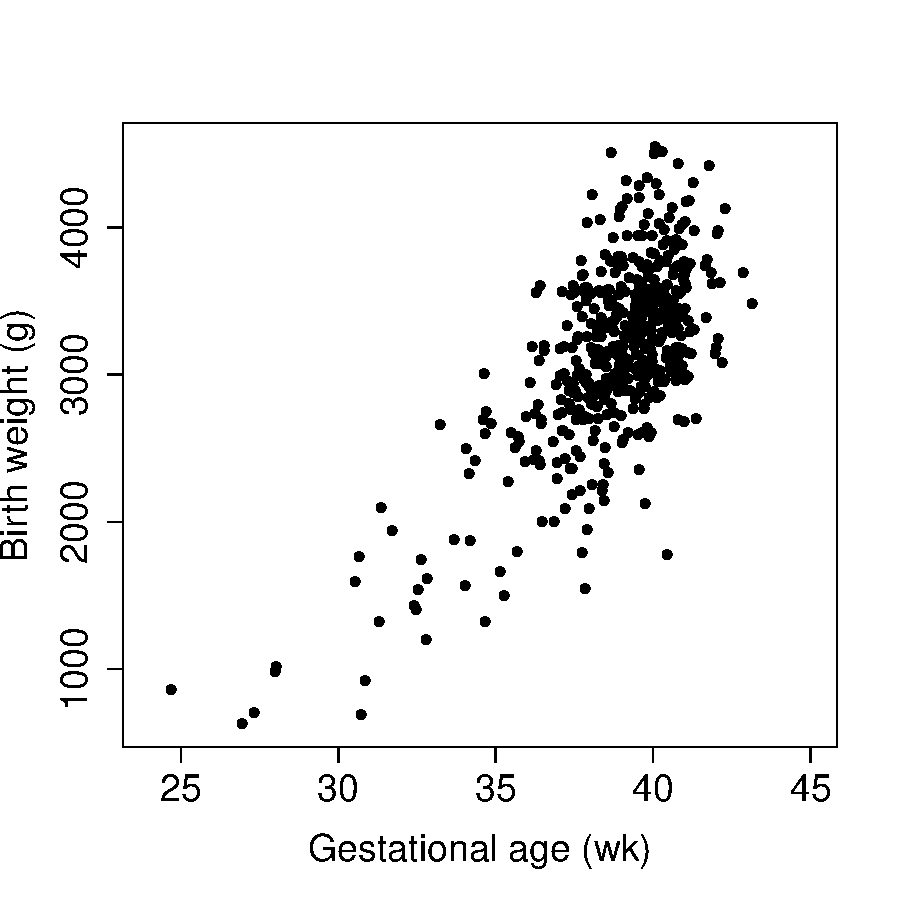
\includegraphics[height=0.75\textheight,keepaspectratio]{lm-bw-by-gw}
\ \\[-2em]
{\small
\begin{Schunk}
\begin{Sinput}
> with(births, plot(bweight ~ gestwks, xlim = c(24,45), pch = 16, cex.axis=1.5, cex.lab = 1.5, 
+  xlab= "Gestational age (wk)", ylab= "Birth weight (g)" ) )
\end{Sinput}
\end{Schunk}
}			

\end{frame}


\begin{frame}[fragile]\frametitle{Metric response, numeric explanatory variable}

% Assuming that the
Roughly linear relationship btw \texttt{bweight}
and \texttt{gestwks} 

$\to$ 
 Simple {\bf linear regression model} fitted.
\begin{semiverbatim}
> m <- lm(bweight ~ gestwks, data=births)
\end{semiverbatim}
\begin{itemize}
\item \texttt{lm()} is the function that fits linear regression models,
assuming \\ {\bf Gaussian} distribution or \textbf{family} for {\bf error} terms.
\medskip
\item \verb+bweight ~ gestwks+ is the {\bf model formula}
\medskip
\item \texttt{m} is a {\bf model object} belonging to {\bf class} ``{\tt lm}''.
\end{itemize}

\medskip

\verb|> coef(m)| -- Printing the estimated regression coefficients
{\small
\begin{semiverbatim}
(Intercept)     gestwks 
    -4489.1       197.0 
\end{semiverbatim}
}
Interpretation of {\bf intercept} and {\bf slope}?
% : ``Each additional week of gestation produces on average 
% an extra 197g''. -- {\it What about the intercept?}
\vfill
\end{frame}


\begin{frame}[fragile]\frametitle{Model object and extractor functions}

Model object = {\bf list} of different elements, each being
separately accessible. \\ -- See \texttt{str(m)} for the full list.

\medskip
Functions that extract results from the fitted model object

\bi
\item
 \verb|summary(m)| -- lots of output
\medskip
\item
\verb|coef(m)| -- beta-hats only (see above)
%% {\small
%% \begin{verbatim}
%% (Intercept)     gestwks 
%%     -4489.1      197.0 
%% \end{verbatim}
%% }
\medskip
\item
\verb|ci.lin(m)[,c(1,5,6)]| -- $\widehat\beta_j$s plus confidence limits 
{\small
\begin{verbatim}
            Estimate    2.5%   97.5%
(Intercept)  -4489.1 -5157.3 -3821.0
gestwks        197.0   179.7   214.2
\end{verbatim}
}
Function \texttt{ci.lin()} is found in {\tt Epi} package.
\medskip
\item
\verb|anova(m)| -- Analysis of Variance Table

\ei
\end{frame}




\begin{frame}[fragile]\frametitle{Other extractor functions, for example}

\bi
\item \texttt{fitted(m), resid(m), vcov(m),} \dots 
\medskip
\item \texttt{predict(m, newdata = ..., interval=...)} 
\bi
{\normalsize
\item[--] Predicted responses for desired combinations 
of new values of the regressors -- {\tt newdata}
\medskip
\item[--] Argument {\tt interval} specifies whether \\
{\bf confidence} intervals for the {\it mean} response or \\ {\bf prediction} intervals
for {\it individual} responses \\ are returned.
}
\ei
% \medskip
\item \texttt{plot(m)} -- produces various diagnostic plots based
on residuals \\ (raw, standardized or studentized residuals).
\ei

Many of these are special {\bf methods} for certain {\bf generic functions},  
aimed at acting on objects of class ``{\tt lm}''.  
%% (For other classes, generic functions mostly act differently.) 

 
\vfill
\end{frame}



\begin{frame}[fragile]
\frametitle{Fitted values, confidence \& prediction intervals}
%% \ \\[-3em]
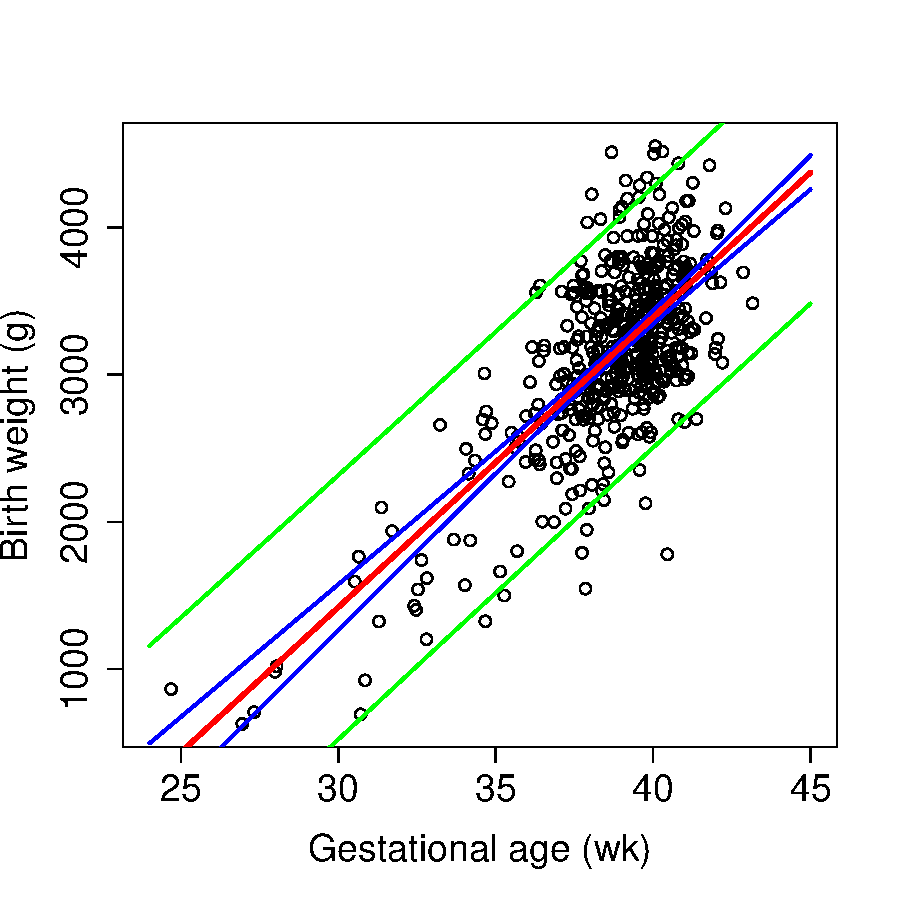
\includegraphics[height=0.65\textheight,keepaspectratio]{lm-bw-by-gw-pr1}
\ \\[-2em]
{\scriptsize
\begin{Schunk}
\begin{Sinput}
> nd <- data.frame( gestwks = seq(24, 45, by = 0.25 ) )
> pr.c1 <- predict( m, newdata=nd, interval="conf" )
> pr.p1 <- predict( m, newdata=nd, interval="pred" )
> with(births, plot(bweight ~ gestwks, xlim = c(24,45), cex.axis=1.5, cex.lab = 1.5, xlab = 'Gestational age (wk)', ylab = 'Birth weight (g)'   ) )
> matlines( nd$gestwks, pr.c1, lty=1, lwd=c(3,2,2), col=c('red','blue','blue')) 
> matlines( nd$gestwks, pr.p1, lty=1, lwd=c(3,2,2), col=c('red','green','green'))
\end{Sinput}
\end{Schunk}
}
\end{frame}



\begin{frame}[fragile]
\frametitle{A couple of diagnostic plots}
%% \ \\[-2em]
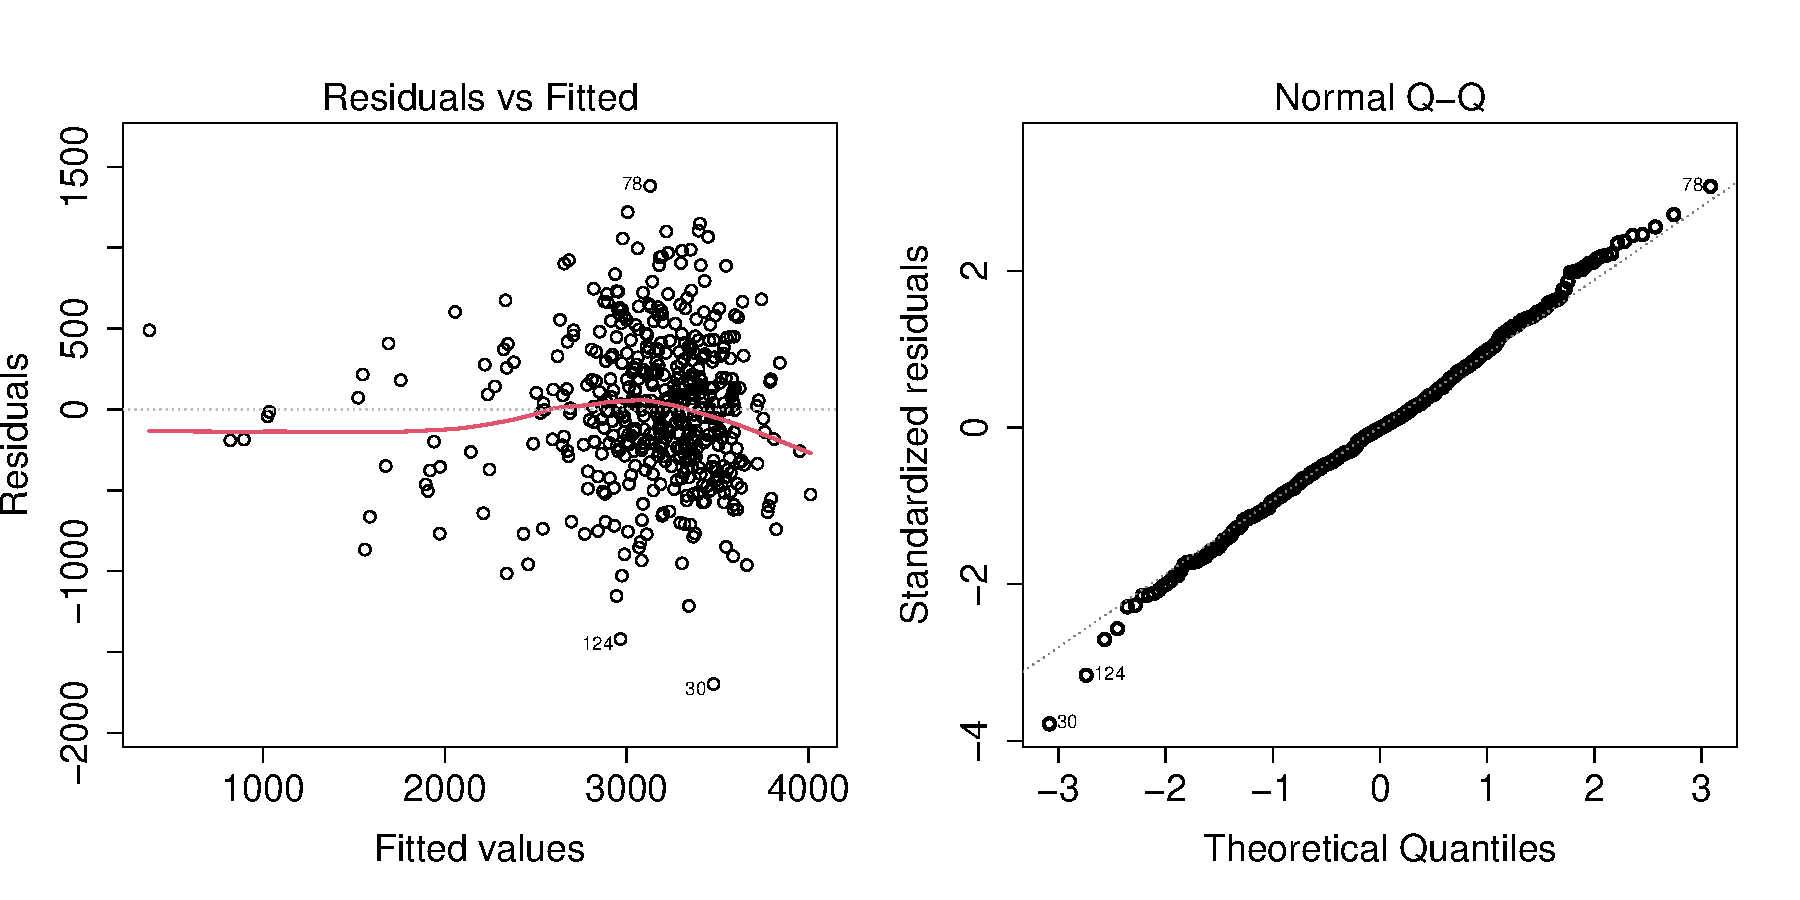
\includegraphics[height=0.65\textheight,width=1.3\textheight, keepaspectratio ]{lm-bw-by-gw-diag}
\ \\[-2em]
\begin{Schunk}
\begin{Sinput}
> par(mfrow=c(1,2))
> plot(m, 1:2, cex.lab = 1.5, cex.axis=1.5, cex.caption=1.5, lwd=2)
\end{Sinput}
\end{Schunk}
\bi
\item Some deviation from linearity?
\item Reasonable agreement with Gaussian error assumption?
\ei

\end{frame}






\begin{frame}[fragile]
\frametitle{Factor as an explanatory variable}

\bi
\item How \texttt{bweight} depends on maternal hypertension?
\begin{semiverbatim}
> mh <- lm( bweight ~ hyp, data=births)}

            Estimate   2.5%  97.5%
(Intercept)   3198.9 3140.2 3257.6
hypH          -430.7 -585.4 -275.9
\end{semiverbatim}
}

\medskip
\item Removal of intercept $\to$ mean \texttt{bweight}s by {\tt hyp}:
%  at the two levels of \texttt{hyp}.
{\small
\begin{semiverbatim}
> mh2 <- lm( bweight ~ -1 + hyp, data = births)
> coef(mh2)
  hypN   hypH 
3198.9 2768.2 
\end{semiverbatim}
}

\medskip
\item
Interpretation: {\tt -430.7 = 2768.2 - 3198.9} \\ 
= difference between level 2 (``\texttt{H}'') {\it vs.} 
reference level 1 (``\texttt{N}'') of factor {\tt hyp}.
\ei
\vfill
\end{frame}

\begin{comment}

\begin{frame}[fragile]\frametitle{Additive model with both {\tt gestwks} and {\tt hyp}}

\medskip

\setlength{\unitlength}{2000sp}%
%
\begingroup\makeatletter\ifx\SetFigFont\undefined%
\gdef\SetFigFont#1#2#3#4#5{%
  \reset@font\fontsize{#1}{#2pt}%
  \fontfamily{#3}\fontseries{#4}\fontshape{#5}%
  \selectfont}%
\fi\endgroup%
\begin{picture}(8649,5862)(1114,-6661)
\thinlines
{\color[rgb]{0,0,0}\put(1126,-6211){\line( 1, 0){7725}}
}%
{\color[rgb]{0,0,0}\put(1726,-5161){\line( 2, 1){6180}}
}%
{\color[rgb]{0,0,0}\put(3901,-4936){\line( 2, 1){5940}}
}%
{\color[rgb]{0,0,0}\put(1126,-6211){\line( 0, 1){5400}}
}%
\put(7726,-6661){\makebox(0,0)[lb]{\smash{{\SetFigFont{12}{14.4}{\rmdefault}{\mddefault}{\updefault}{\color[rgb]{0,0,0}gestwks}%
}}}}
\put(1951,-5386){\makebox(0,0)[lb]{\smash{{\SetFigFont{12}{14.4}{\rmdefault}{\mddefault}{\updefault}{\color[rgb]{0,0,0}A}%
}}}}
\put(4051,-5386){\makebox(0,0)[lb]{\smash{{\SetFigFont{12}{14.4}{\rmdefault}{\mddefault}{\updefault}{\color[rgb]{0,0,0}B}%
}}}}
\put(1426,-1111){\makebox(0,0)[lb]{\smash{{\SetFigFont{12}{14.4}{\rmdefault}{\mddefault}{\updefault}{\color[rgb]{0,0,0}Birth weight}%
}}}}
%\put(4276,-3211){\makebox(0,0)[lb]{\smash{{\SetFigFont{12}{14.4}{\rmdefault}{\mddefault}{\updefault}{\color[rgb]{0,0,0}hyp = normal}%
\put(3200,-3211){\makebox(0,0)[lb]{\smash{{\SetFigFont{12}{14.4}{\rmdefault}{\mddefault}{\updefault}{\color[rgb]{0,0,0}hyp = normal}%
}}}}
\put(6751,-3811){\makebox(0,0)[lb]{\smash{{\SetFigFont{12}{14.4}{\rmdefault}{\mddefault}{\updefault}{\color[rgb]{0,0,0}hyp = hyper}%
}}}}
\end{picture}%

The effect of {\tt gestwks} is the slope of the lines A and B, which is assumed to be the
same. The effect of {\tt hyp} is the constant vertical distance between the lines.

\end{frame}

\end{comment}

\begin{frame}[fragile]\frametitle{Additive model with both gestwks and hyp}
%% Multiple regression: {\tt gewtwks} and {\tt hyp}}

%% An additive model for {\tt bweight} including both
\bi
\item
Joint effect of
 \texttt{hyp} and \texttt{gestwks} % under additivity
 is modelled e.g. by updating: % a simpler model:

\medskip
\verb|> mhg <- update(mh, . ~ . + gestwks)|
{\small
\begin{semiverbatim}
            Estimate    2.5%   97.5%
(Intercept)  -4285.0 -4969.7 -3600.3
hypH          -143.7  -259.0   -28.4
gestwks        192.2   174.7   209.8
\end{semiverbatim}
}
\medskip
\item
The coefficient for {\tt hyp}: {\tt H} {\it vs.} {\tt N}
 is attenuated (from $-430.7$ to $-143.7$). 
\medskip
\item 
Does $-143.7$ estimate the \textbf{causal effect} of \texttt{hyp}
\textbf{adjusted} for \texttt{gestwks}?
\medskip
\item
No, as \texttt{gestwks} is most likely a \textbf{mediator}. --  
Much of the effect of \texttt{hyp} on 
\texttt{bweight} is mediated via
shorter \texttt{gestwks} in hypertensive mothers.
\medskip
\item
Instead, for \textbf{total causal effect} of \texttt{hyp}, 
adjustment for at least age is needed, but adjusting for \texttt{gestwks}
is \textbf{overadjustment}. 
\medskip
\item
Yet, for \textbf{predictive
modelling} it is OK to keep \texttt{gestwks}. 
\ei

% \vfill

\end{frame}

\begin{comment}

\begin{frame}[fragile]\frametitle{Interaction between {\tt hyp} and {\tt gestwks}}

\medskip

\setlength{\unitlength}{2000sp}%
%
\begingroup\makeatletter\ifx\SetFigFont\undefined%
\gdef\SetFigFont#1#2#3#4#5{%
  \reset@font\fontsize{#1}{#2pt}%
  \fontfamily{#3}\fontseries{#4}\fontshape{#5}%
  \selectfont}%
\fi\endgroup%
\begin{picture}(8199,6105)(889,-6661)
\thinlines
{\color[rgb]{0,0,0}\put(901,-6361){\line( 0, 1){5700}}
}%
{\color[rgb]{0,0,0}\put(901,-6361){\line( 1, 0){8175}}
}%
{\color[rgb]{0,0,0}\put(2101,-4936){\line( 4, 3){5064}}
}%
{\color[rgb]{0,0,0}\put(3151,-5611){\line( 6, 1){5594.595}}
}%
\put(1201,-736){\makebox(0,0)[lb]{\smash{{\SetFigFont{12}{14.4}{\rmdefault}{\mddefault}{\updefault}{\color[rgb]{0,0,0}Birth weight}%
}}}}
\put(6976,-6661){\makebox(0,0)[lb]{\smash{{\SetFigFont{12}{14.4}{\rmdefault}{\mddefault}{\updefault}{\color[rgb]{0,0,0}gestwks}%
}}}}
\put(3000,-2536){\makebox(0,0)[lb]{\smash{{\SetFigFont{12}{14.4}{\rmdefault}{\mddefault}{\updefault}{\color[rgb]{0,0,0}hyp = normal}%
}}}}
%\put(7426,-4786){\makebox(0,0)[lb]{\smash{{\SetFigFont{12}{14.4}{\rmdefault}{\mddefault}{\updefault}{\color[rgb]{0,0,0}hyp = hyper}%
\put(7426,-5200){\makebox(0,0)[lb]{\smash{{\SetFigFont{12}{14.4}{\rmdefault}{\mddefault}{\updefault}{\color[rgb]{0,0,0}hyp = hyper}%
}}}}
%\put(4426,-4111){\makebox(0,0)[lb]{\smash{{\SetFigFont{12}{14.4}{\rmdefault}
%{\mddefault}{\updefault}{\color[rgb]{0,0,0}Strata}%
%}}}}
\end{picture}%

The effect of {\tt hyp} increases

\end{frame}

\end{comment}

\begin{frame}[fragile]
\frametitle{Model with interaction of {\tt hyp} and {\tt gestwks}}

\bi
\item
% A model including an interaction upon the main effects: \\
%\begin{verbatim}
{\small \verb|mhgi <- lm(bweight ~ hyp + gestwks + hyp:gestwks, ...)|
\medskip
\item
Or with shorter formula: {\small \verb| bweight ~ hyp * gestwks |}
{\small
\begin{verbatim}
              Estimate    2.5%   97.5%
(Intercept)    -3960.8 -4758.0 -3163.6
hypH           -1332.7 -2841.0   175.7
gestwks          183.9   163.5   204.4
hypH:gestwks      31.4    -8.3    71.1
\end{verbatim}
}
\medskip
\item
Estimated slope: 183.9 g/wk in reference group {\tt N} of normotensive mothers and \\
 183.9 + 31.4 = \ 215.3 g/wk in hypertensive mothers.
\medskip
\item[$\Leftrightarrow$]
% Interpretation of {\tt hypH:gestwks}: \\
% \bi
% {\normalsize
% \item[ ] 
For each additional week the difference
in mean {\tt bweight} between 
{\tt H} and {\tt N} group
 increases by 31.4 g.
% \ei
\medskip
\item
{\it Interpretation of \verb| Intercept| and ``main effect'' \verb| hypH|?}
\ei
\end{frame}

\begin{frame}[fragile]
\frametitle{Model with interaction (cont'd)}

More interpretable parametrization 
obtained if {\tt gestwks} is {\bf centered}
at some reference value, using e.g.
the {\bf insulate} operator {\tt I()} for explicit  
transformation of an original term.
\bi
\item {\small \verb|mi2 <- lm(bweight ~ hyp*I(gestwks-40), ...)|}
{\small  
\begin{verbatim}
                     Estimate   2.5%  97.5%
(Intercept)            3395.6 3347.5 3443.7
hypH                    -77.3 -219.8   65.3
I(gestwks - 40)         183.9  163.5  204.4
hypH:I(gestwks - 40)     31.4   -8.3   71.1
\end{verbatim} 
}
\medskip
\item
The ``main effect'' of {\tt hyp} = $-77.3$ is the % effect of {\tt hyp} 
difference between
{\tt H} and {\tt N} \\ at the reference value 
{\tt gestwks} = 40.
\medskip
\item
{\tt Intercept} = 3395.6 is the estimated mean {\tt bweight} \\ at 
the reference value 40 of {\tt gestwks} in {\tt group N}.

\ei

\end{frame}



\begin{frame}
\frametitle{Factors and contrasts in R}

\bi
\item
A categorical explanatory variable or {\bf factor}  
with $L$ {\bf levels} will be represented by $L-1$ linearly independent
columns in the \\ {\bf model matrix} of a linear model. 
\medskip
\item
These columns can be defined in various ways implying
alternative {\bf parametrizations} for the effect of the factor.
\medskip
\item 
Parametrization is defined by given type of {\bf contrasts}. 
\medskip
\item 
Default: {\bf treatment} contrasts, in which 1st class is the {\bf reference}, 
and regression coefficient $\beta_k$ for class $k$ is interpreted as $\beta_k = \mu_k - \mu_1$
\medskip
\item
Own parametrization may be tailored by
function {\tt C()}, with the pertinent 
{\bf contrast matrix} as argument.  
\medskip
\item
Or, use {\tt ci.lin(mod, ctr.mat = CM)} after fitting.
\ei
\end{frame}


\begin{comment}

\begin{frame}[fragile]\frametitle{Factors: parametrization and contrasts}

\bi
\item
The {\bf expected response} $\mu$  depends on 
numeric explanatory terms $X, Z, \cdots$ via a {\bf linear predictor} $\eta$
\[
\mu = \eta, \ \text{ where }\ \eta = \alpha+\beta X + \gamma Z + \cdots 
\]
\item 
In many GLMs we put $g(\mu) = \eta$, where $g$ is a suitable {\bf link} function of $\mu$
 -- e.g. \log$(\mu)$ or logit$(\mu)$.
\medskip
\item
When $X$ is a factor, on (say) 3 levels, it is replaced by $X_1, X_2, X_3$, the indicator variables for the levels of $X$.
\medskip
\item
Expected values  $\mu = \alpha+\beta_1 X_1 + \beta_2 X_2 + \beta_3 X_3$ are

\begin{center}
\begin{tabular}{lccccl}
level&${\mathbf 1}$ (i'cept) &$X_1$&$X_2$&$X_3$ & $\mu$ \\ % $\alpha+\beta_1 X_1 + \beta_2 X_2 + \beta_3 X_3$\\
\hline
1&1&1&0&0& $\mu_1 = \alpha+\beta_1$\\
2&1&0&1&0& $\mu_2 = \alpha+\beta_2$\\
3&1&0&0&1& $\mu_3 = \alpha+\beta_3$
\end{tabular}
\end{center}
\ei
\vfill
\end{frame}

\begin{frame}[fragile]
\frametitle{Too many parameters -- model matrix singular!}


\textcolor{blue}{Drop $\alpha$}

\vspace{-2ex}

{\small
\begin{center}
\begin{tabular}{lcccl}
level&$X_1$&$X_2$&$X_3$ &$\mu=\beta_1 X_1 + \beta_2 X_2 + \beta_3 X_3$\\
\hline
1&1&0&0& $\beta_1$\\
2&0&1&0& $\beta_2$\\
3&0&0&1& $\beta_3$
\end{tabular}
\end{center}

$\beta_1$ is the mean response at level~1, $\beta_2$ at level~2, $\beta_3$ at level~3.


\textcolor{blue}{Drop $X_1$} $\to$  {\bf treatment contrasts} (default in R).

% \vspace{-2ex}

\begin{center}
\begin{tabular}{lcccl}
level& ${\mathbf 1}$ & $X_2$ & $X_3$ & $\mu = \alpha+\beta_2 X_2 + \beta_3 X_3$\\
\hline
1 (ref.) & 1 & 0 & 0 & $\mu_1 = \alpha$\\
2& 1 & 1 & 0 & $\mu_2 = \alpha+\beta_2$\\
3& 1 & 0 & 1 & $\mu_3 = \alpha+\beta_3$
\end{tabular}
\end{center}
\bi
\item
$\alpha$ is the mean response at {\bf reference level} 1
\item
$\beta_2 = \mu_2 - \mu_1$ and $\beta_3 = \mu_3-\mu_1$ are the mean differences of 
levels 2 and 3, respectively, {\it vs.} level 1
\ei
The pertinent columns in the model matrix are obtained by multiplying the matrix comprising the indicator columns by
the following {\bf contrast matrix}
\[
{\mathbf M} = [ M_1 \ M_2 ] = 
\left[
\begin{array}{cc}
0&0\\
1&0\\
0&1
\end{array}
\right]
\]
%% }
\vfill
\end{frame}

\end{comment}

\begin{frame}[fragile]\frametitle{Two factors: additive effects}

\bi
\item
Factor $X$ has 3 levels, $Z$ has 2 levels -- Model:
\[
\mu=\alpha+\beta_1 X_1+ \beta_2 X_2+\beta_3 X_3+\gamma_1 Z_1 +\gamma_2 Z_2
\]
\item
$X_1$ (reference), $X_2, X_3$ are the indicators for $X$,  
\medskip
\item
$Z_1$ (reference), $Z_2$ are the indicators for $Z$.
\medskip
\item
Omitting $X_1$ and $Z_1$ the model for mean is:
\[
\mu=\alpha+\beta_2 X_2+\beta_3 X_3 +\gamma_2 Z_2
\]
with predicted means $\mu_{jk}$ ($j=1,2,3; k = 1,2$):
\begin{center}
\begin{tabular}{llll}
&& $Z= 1$ & $Z = 2$ \\
\hline
&1 & $\mu_{11} = \alpha$ & $\mu_{11} = \alpha + \gamma_2$\\
$X$&2 & $\mu_{21} = \alpha+\beta_2$ & $\mu_{22} = \alpha +\beta_2+ \gamma_2$\\
&3 & $\mu_{31}= \alpha+\beta_3$ & $\mu_{32} = \alpha +\beta_3+ \gamma_2$
\end{tabular}
\end{center}
\ei
\vfill

\end{frame}



\begin{frame}[fragile]\frametitle{Two factors with interaction}

\begin{comment}
Effect of $Z$ the same at each level of $X$:

\begin{center}
\begin{tabular}{llcc}
&& $Z = 1$ & $Z=2$\\
\hline
&1 & $\alpha$ & $\alpha + \gamma_2$\\
$X$&2 & $\alpha+\beta_2$ & $\alpha +\beta_2+ \gamma_2$\\
&3 & $\alpha+\beta_3$ & $\alpha +\beta_3+ \gamma_2$
\end{tabular}
\end{center}
\end{comment}

\bi
\item
Effect of $Z$ differs at different  levels of $X$:
\begin{center}
\begin{tabular}{llll  }
&& $Z = 1$ & $Z = 2$ \\
\hline
&1 & $\mu_{11} = \alpha$ & $\mu_{12} = \alpha + \gamma_2$\\
$X$&2 & $\mu_{21} = \alpha+\beta_2$ & $\mu_{22} = \alpha +\beta_2+ \gamma_2+\delta_{22}$\\
&3 & $\mu_{31} = \alpha+\beta_3$ & $\mu_{32} = \alpha +\beta_3+ \gamma_2+\delta_{32}$
\end{tabular}
\end{center}
\medskip
\item
How much the effect of $Z$ (level 2 {\it vs.} 1) \\ changes  when
the level of $X$ is changed  from 1 to 3:
\begin{align*}
   \delta_{32}  & = (\mu_{32} - \mu_{31}) - (\mu_{12} - \mu_{11})  \\
  & = (\mu_{32} - \mu_{12}) - (\mu_{31} - \mu_{11}),
\end{align*}
= how much the effect of  $X$ (level 3 {\it vs.} 1) \\ 
changes when
the level of $Z$ is changed from 1 to 2.
\medskip
\item See the exercise: interaction of {\tt hyp} and {\tt gest4}.
\ei
\end{frame}



\begin{comment}

\begin{frame}[fragile]
\frametitle{Nested or stratified effects}
A slightly different way of parameterizing the model gives
stratified effects:

\begin{center}
\begin{tabular}{llcc  }
&&\multicolumn{2}{c}{$Z$}\\
&& 1 & 2\\
\hline
&1 & $\beta_1$ & $\beta_1 + \delta_{12}$\\
$X$&2 & $\beta_2$ & $\beta_2+ \delta_{22}$\\
&3 & $\beta_3$ & $\beta_3+\delta_{32}$
\end{tabular}
\end{center}

Same number of parameters as for interaction, but the $\delta$'s  now measure the effects of $Z$ at each level of $X$. In R this would be produced by the model formula \verb@Y ~ -1 + X + X:Z@
\vfill
\end{frame}


\begin{frame}[fragile]\frametitle{Alternatives to treatment contrasts}

You can't put all the indicator variables for a factor into a model with an intercept. Omitting the indicator for level~1 gives contrasts which compares each level with level~1. 

The way this is actually done is by multiplying the matrix composed of all indicator variables by a {\it contrast} matrix to give the model matrix which goes into the model. 

For treatment contrasts the contrast matrix is
\[
\left(
\begin{array}{cc}
0&0\\
1&0\\
0&1
\end{array}
\right)
\]
The corresponding model matrix is essentially the same as the contrast matrix but has one row per subject: $(0 \;\; 0)$ for subjects at level~1, $(1 \;\; 0)$ for subjects at level~2, and $(0 \;\; 1)$ for subjects at level~3.
\end{frame}




\begin{frame}[fragile]
\frametitle{Common contrasts and contrast matrices}

A given contrast matrix ${\mathbf M} = [M_1 \ M_2]$ produces a specific type of
contrasts or parametrization. Three common ones:

\medskip
{\small
\begin{tabular}{cccllr}
level & $M_1$ & $M_2$ & $\mu=\alpha+\beta_1 M_1+\beta_2 M_2$&{\bf Treatment contrasts}\\
\hline
1& 0&0& $\mu_1=\alpha$ &$\alpha=\mu_1$\\
2& 1&0& $\mu_2=\alpha+\beta_1$&$\beta_1=\mu_2-\mu_1$\\
3& 0&1& $\mu_3=\alpha+\beta_2$&$\beta_2=\mu_3-\mu_1$
\end{tabular}

\begin{tabular}{crrllr}
level & $M_1$ & $M_2$ & $\mu=\alpha+\beta_1 M_1+\beta_2 M_2$&{\bf Sum contrasts}\\
\hline
1& 1&0& $\mu_1=\alpha+\beta_1$ &$\alpha=\bar{\mu}$\\
2& 0&1& $\mu_2=\alpha+\beta_2$&$\beta_1=\mu_1-\bar{\mu}$\\
3& $-1$&$-1$& $\mu_3=\alpha-\beta_1-\beta_2$&$\beta_2=\mu_2-\bar{\mu}$
\end{tabular}

\begin{tabular}{cccllr}
level & $M_1$ & $M_2$ & $\mu=\alpha+\beta_1 M_1+\beta_2 M_2$&{\bf Cumulative contrasts}\\
\hline
1& 0&0& $\mu_1=\alpha$&$\alpha=\mu_1$\\
2& 1&0& $\mu_2=\alpha+\beta_1$&$\beta_1=\mu_2-\mu_1$\\
3& 1&1& $\mu_3=\alpha+\beta_1+ \beta_2$&$\beta_2=\mu_3-\mu_2$
\end{tabular}


}
\end{frame}

\end{comment}

\begin{frame}[fragile]

\frametitle{Contrasts in \R}

\bi
%% \item
%% Default: treatment contrasts  ({\tt contr.treatment}). 
%% \medskip
%% \item
%% For ordered factors the default is  polynomial contrasts ({\tt contr.poly}; somewhat difficult to interpret). 
%% \medskip
\item
All contrasts can be implemented by supplying a suitable
{\bf contrast function} giving the {\bf contrast matrix} e.g:
{\small
\begin{semiverbatim}
{> contr.cum(3)}        {> contr.sum(3)}
1 0 0                  1    1   0    
2 1 0                  2    0   1   
3 1 1                  3   -1  -1   
\end{semiverbatim}
}
\medskip
\item
In model formula factor name {\tt faktori} can be replaced by expression
like \verb+C(faktori, contr.cum)+.
\medskip
\item 
Function \texttt{ci.lin()} can calculate CI's for
linear functions of the parameters of a fitted
model {\tt mall} when supplied by a relevant contrast matrix \\
\verb|> ci.lin(mall, ctr.mat = CM)[ , c(1,5,6)]|

\medskip
$\to$ No need to specify contrasts in model formula!
\ei
\end{frame}



\begin{comment}

\begin{frame}[fragile] \frametitle{Exploring contrasts}
A good way to explore contrasts is to use a simple data set:
{\small
\begin{semiverbatim}
{\color{DarkGreen}
> y <- c(1,2,5,4)
> x <- factor(1:4)

> lm(y ~ x)}
(Intercept)           x2           x3           x4  
          1            1            4            3  

{\color{DarkGreen}> lm(y ~ C(x,contr.cum))}
     (Intercept)  C(x, cum)2  C(x, cum)3  C(x, cum)4  
               1           1           3          -1  

{\color{DarkGreen}> lm(y ~ C(x,contr.sum))}
     (Intercept)  C(x, sum)1  C(x, sum)2  C(x, sum)3  
               3          -2          -1           2 
\end{semiverbatim}
}
\end{frame}



\begin{frame}[fragile] 
\frametitle{Using {\tt ci.lin()} to calculate contrasts}

Function \texttt{ci.lin()} has an option for calculating CI's for
linear functions of the parameters of a fitted
model. 

Using \texttt{gest4} as an example, first fit a model omitting
the intercept:
\begin{semiverbatim}
\color{DarkGreen}> m <- lm(bweight ~ -1 + gest4,data=births)
\end{semiverbatim}
To calculate the linear function $-\mu_1-\mu_2+\mu_3+\mu_4$  create a $1\times$4
matrix with
\begin{semiverbatim}
\color{DarkGreen}> CM <- cbind(-1,-1,1,1)
\end{semiverbatim}
and then use 
\begin{semiverbatim}
{\color{DarkGreen}> ci.lin(m,ctr.mat=CM)[,c(1,5,6)]}

Estimate     2.5\%    97.5\% 
2170.974 1917.045 2424.903 
\end{semiverbatim}

\end{frame}

\end{comment}




\begin{frame}[fragile]\frametitle{More about numeric regressors}

What if dependence of $Y$ on $X$ is non-linear?

\begin{itemize}
\item {\bf Categorize} the values of $X$ into a factor.

\bi
{\normalsize
\item[--] Continuous effects violently discretized 
  by often arbitrary cutpoints. This is inefficient.
}
\ei
\medskip
\item Fit a low-degree (e.g. 2 to 4) {\bf polynomial} of $X$.
\bi
{\normalsize
\item[--] Tail behaviour may be problematic. 
}
\ei
 \medskip
\item Use {\bf fractional polynomials}.
\bi
{\normalsize
\item[--] Invariance problems. Only useful if $X = 0$ is well-defined.
}
\ei
\medskip
\item Use a {\bf spline} model: smooth function $s(X;\beta)$. -- See Martyn's lecture
\bi
{\normalsize
\item[--] More flexible models that act locally.
\item[--] Effect of $X$ reported by graphing $\widehat s(X;\beta)$ \& its CI
}
\ei
\end{itemize}
 
\end{frame}



\begin{frame}[fragile]
\frametitle{Mean {\tt bweigth} as 3rd order polynomial of {\tt gestwks}}
\ \\[-3em]
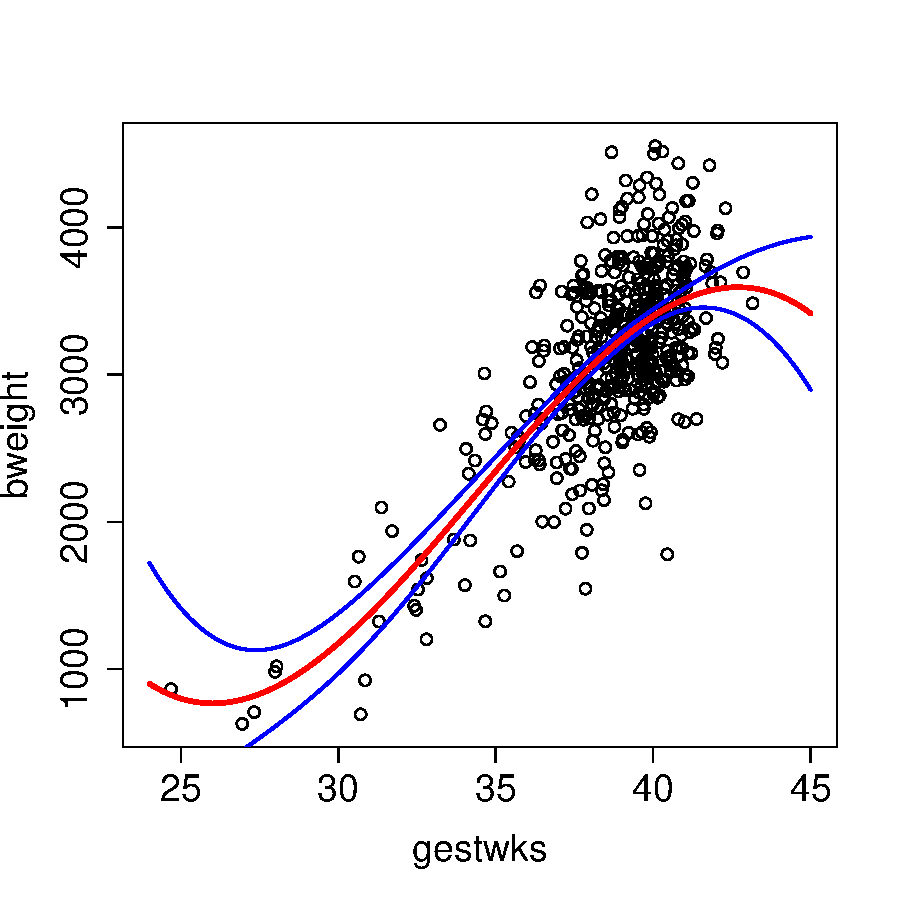
\includegraphics[height=0.70\textheight,keepaspectratio]{lm-mp3plot}
\ \\[-2em]
{\small
\begin{Schunk}
\begin{Sinput}
> mp3 <- update( m, . ~ . - gestwks + poly(gestwks, 3) )  
\end{Sinput}
\end{Schunk}
}
\ \\[-2em]
\begin{itemize}
\item The model is linear in parameters with 4 terms \& 4 df.
\item Otherwise good, but the tails do not behave well.
\end{itemize}

}
\end{frame}

\begin{comment}

\begin{frame}[fragile]
\frametitle{Natural regression spline model: 10 knots}
\ \\[-3em]
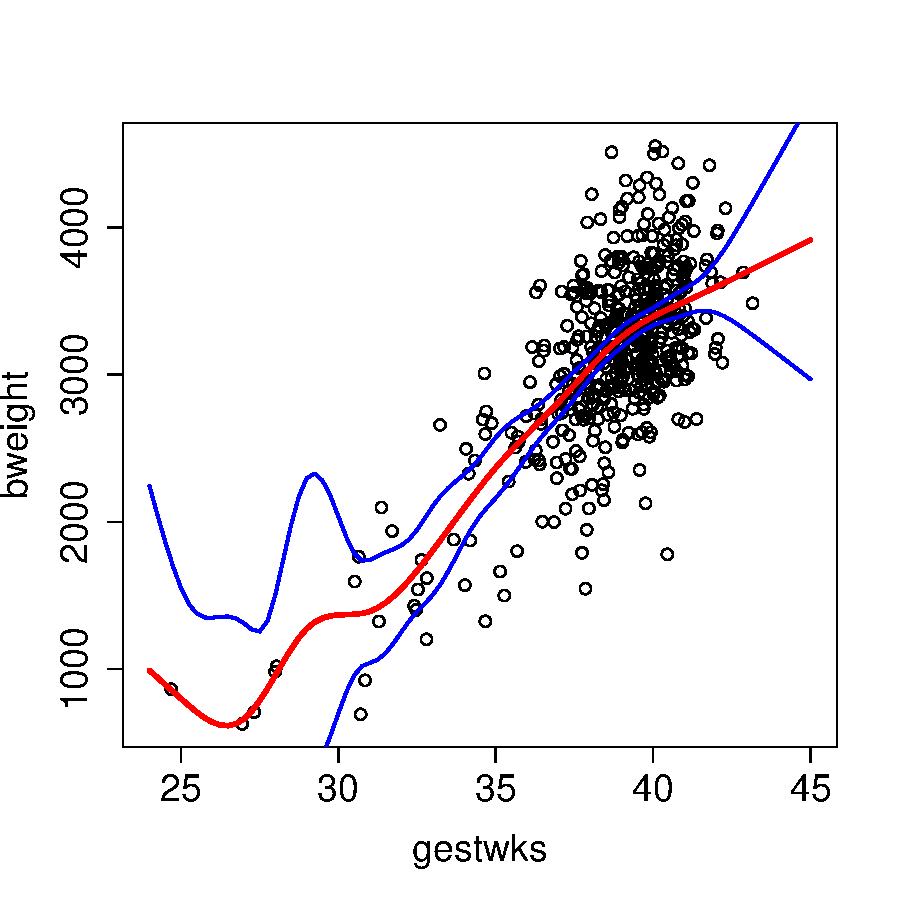
\includegraphics[height=0.70\textheight,keepaspectratio]{lm-mNs10-plot}
\ \\[-2em]
{\small
\begin{Schunk}
\begin{Sinput}
> mNs10 <- lm( bweight ~ Ns( gestwks, 
+       knots = seq(25, 43, by = 2)), data = births)
\end{Sinput}
\end{Schunk}
}
\ \\[-2em]
\begin{itemize}
\item Perhaps too flexible \dots
\end{itemize}

\end{frame}


\begin{frame}[fragile]
\frametitle{Natural regression spline model:  2 knots}
\ \\[-3em]
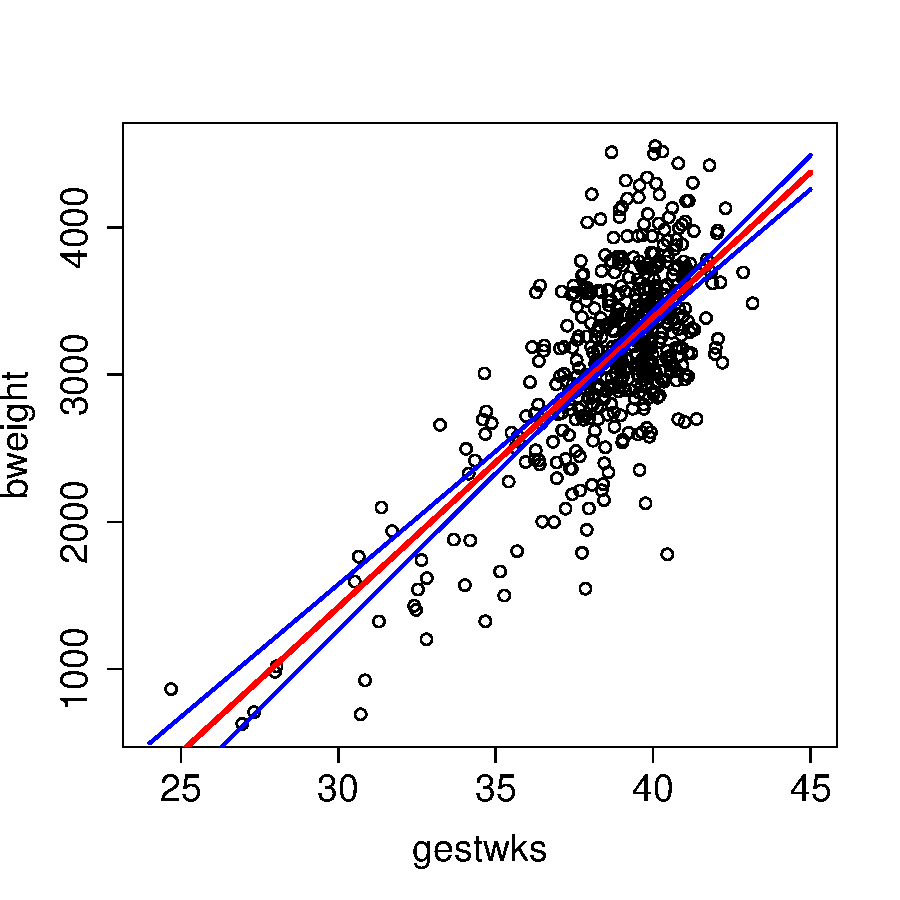
\includegraphics[height=0.70\textheight,keepaspectratio]{lm-mNs2-plot}
\ \\[-2em]
{\small
\begin{Schunk}
\begin{Sinput}
> mNs2 <- lm( bweight ~ Ns( gestwks, 
+       knots = c(37, 41)), data = births)
\end{Sinput}
\end{Schunk}
}

\ \\[-2em]
\begin{itemize}
\item Perhaps too rigid \dots
\end{itemize}

\end{comment}

\end{frame}
\begin{frame}[fragile]
\frametitle{Penalized spline model with cross-validation}
\ \\[-3em]
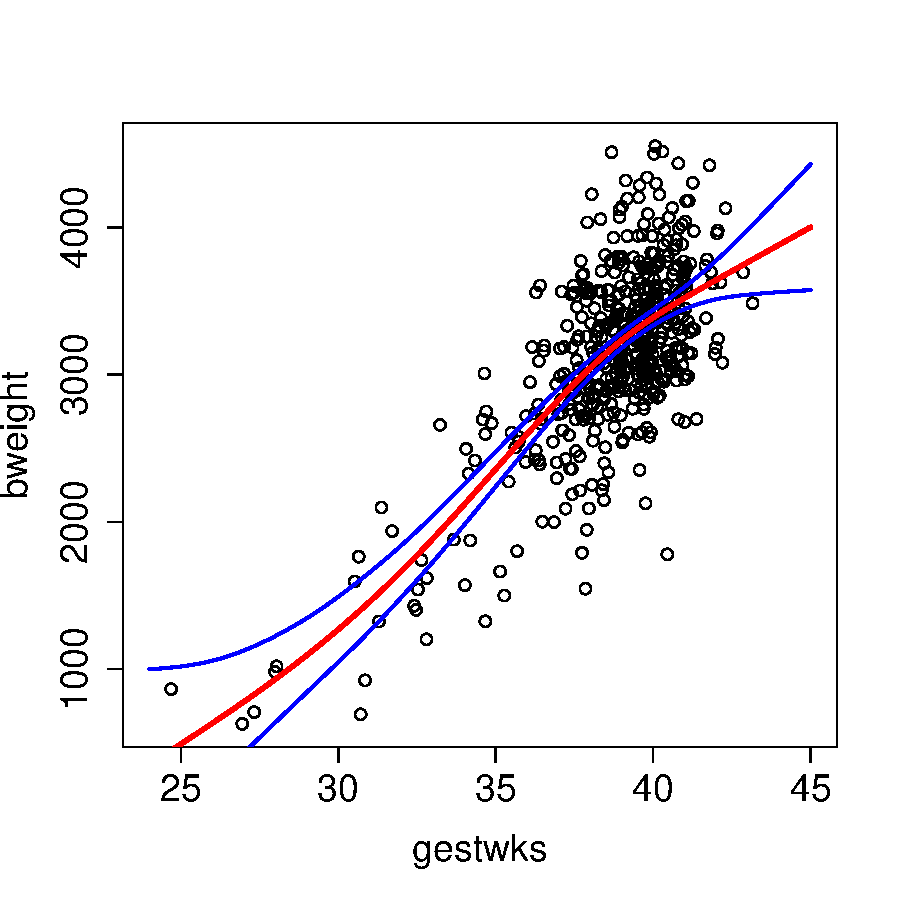
\includegraphics[height=0.70\textheight,keepaspectratio]{lm-mPen-plot}
\ \\[-3em]
{\small
\begin{Schunk}
\begin{Sinput}
> library(mgcv)
> mpen <- gam( bweight ~ s(gestwks), data = births)
\end{Sinput}
\end{Schunk}
}
\ \\[-2em]
\begin{itemize}
\item Looks quite nice.
\item Model df $\approx 4.2$; close to $4$, as in the 3rd degree polynomial model.
\end{itemize}


\end{frame}

\begin{comment}

\begin{frame}[fragile]
\frametitle{Diagnostics of the penalized spline model}
\ \\[-2em]
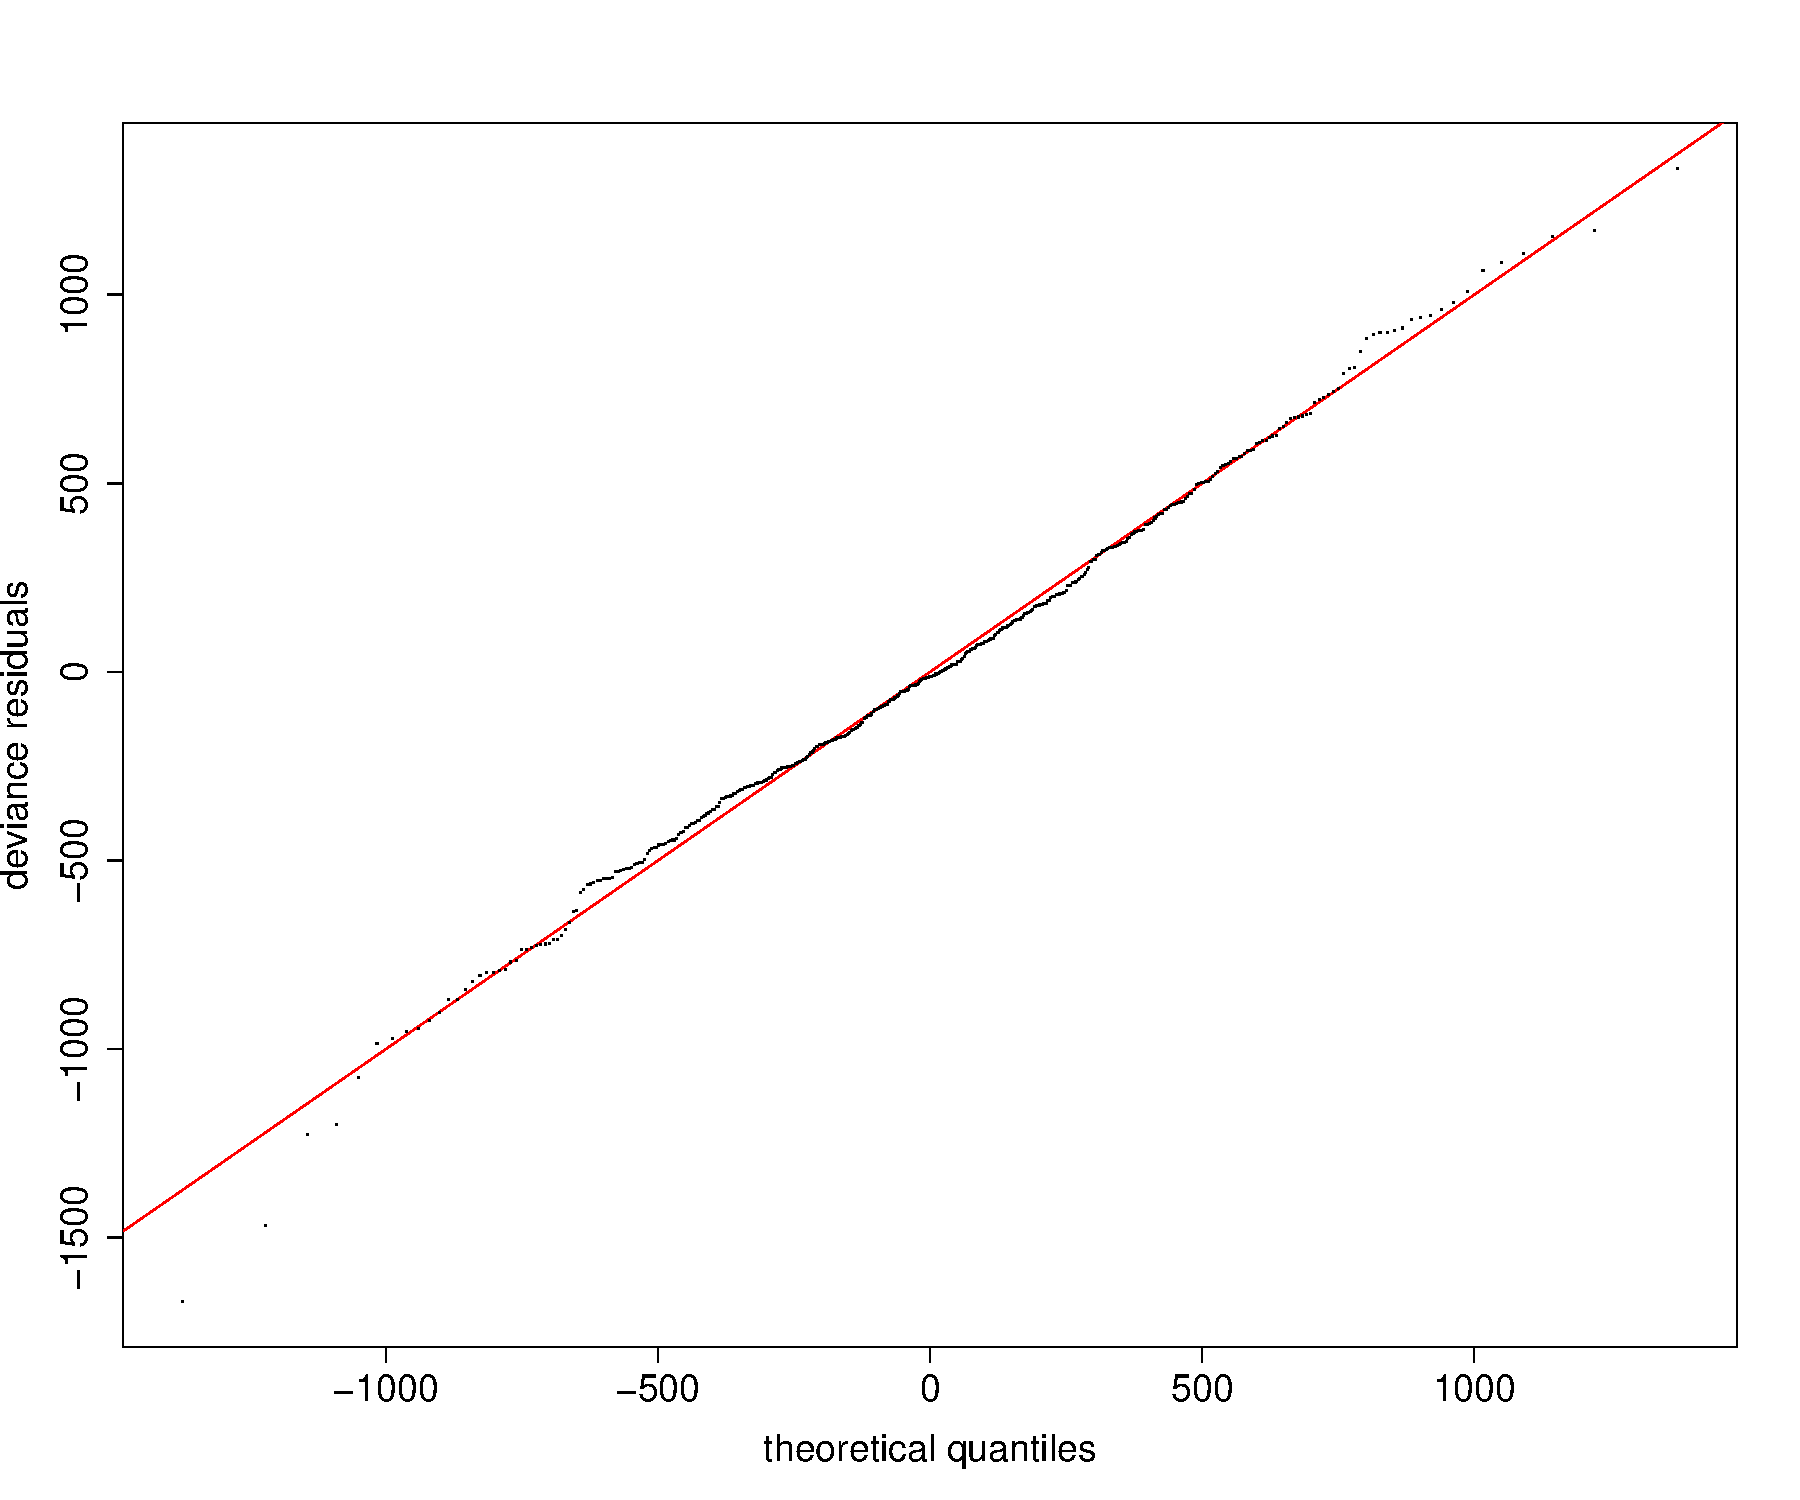
\includegraphics[height=0.65\textheight,width=1.3\textheight, keepaspectratio ]{lm-bw-by-gw-spline-diag}
\ \\[-2em]
\begin{Schunk}
\begin{Sinput}
> gam.check(mpen, cex.lab = 1.5, cex.axis=1.5, cex.caption=1.5, lwd=2)
\end{Sinput}
\end{Schunk}
\bi
\item Good agreement with the fitted spline curve?
%% \item Reasonable agreement with Gaussian error assumption?
\ei

\end{frame}

\end{comment}

\begin{comment}
%----------------------------------------------------------------------
\begin{frame}[fragile]\frametitle{Fractional polynomials}

$\alpha + \beta_1 x +\gamma_1 x^{-1}$\\
$\alpha + \beta_1 x +\gamma_1 x^{-1} + \beta_2 x^2+\gamma_2 x^{-2}$\\
etc.

A $\log(x)$ term and fractional powers can also be included.
\begin{itemize}
\item The model-matrix is columns of powers of $x$:
{\small
\begin{verbatim}
  > outer( x, -2:2, "^" )
\end{verbatim}
}
\item A model matrix can be inserted directly into a formula:
{\small
\begin{verbatim}
  > lm( y ~ outer( x, -2:2, "^" ) )
\end{verbatim}
}
\end{itemize}

\end{frame}

\end{comment}

\begin{comment}

\begin{frame}[fragile]
  \frametitle{What is a spline?}
\begin{minipage}[t]{0.50\textwidth}
\raggedright
\begin{itemize}
\item Piecewise polynomial \\ -- typically cubic.
\medskip
\item Pieces joined together at $K$ {\bf knots}.
\medskip
\item 0th, 1st and 2nd derivatives  
 continuous even at knots.
\medskip
\item $s(X;\beta)$ is linear in $\beta$ parameters for
intercept, 1st, 2nd and 3rd order terms of $X$, plus
$K$ truncated cubic terms. Total $4 + K$ 
coefficients.

\end{itemize}
\end{minipage}
\hspace*{1ex}
\begin{minipage}[t]{0.45\textwidth}
\ \\[-1ex]
\includegraphics[width=1.1\textwidth]{csp}
\end{minipage}

\end{frame}

\begin{frame}
\frametitle{Regression spline}
\begin{itemize}
\item User specifies no. ($K$) and location of knots, which define the
  truncated cubic terms in the model matrix or {\bf basis}
\medskip
\item {\bf Natural spline}: the curve forced to be linear 
beyond the extreme knots $\Rightarrow$ 
 Model df = $K$
\medskip
\item The results depend heavily on choice of $K$ and locations -- How to choose them?
\end{itemize}
R package \texttt{splines}.
\begin{\itemize}
\item \texttt{bs(x, knots = ...)}: {\bf basic} splines, any degree.
\item\texttt{ns()}:  {\bf natural} cubic splines. 
%% -- cubic splines constrained to be  linear beyond the boundary knots. 
\item\texttt{Ns()}: wrapper of {\tt ns()} in {\tt Epi} \\
 -- convenient with time-split epidemiologic data.	
\item If knots not given, but df is, they are computed from data.
\end{itemize}

\end{frame}

\begin{frame}
\frametitle{Penalized spline}
\begin{itemize}
\item $s(X, \beta)$ is defined as a regression spline with 
the basis dimension $K$ allowed to be quite large (10 to 40) 
\medskip
\item Parameters $\beta$ estimated by {\bf penalized least squares} \\
 -- minimize the following w.r.t $\beta$:
$$ \sum_{i=1}^n \{ Y_i - s(X_i; \beta) \}^2 \ + \ 
     \lambda \int %% _{\min \{ X_i\} }^{\max \{X_i\} } 
		   s''(x; \beta)dx, $$
\item The latter term is {\bf penalty} for roughness of $s(X; \beta)$.
\medskip
\item $\lambda$ determines the degree of smoothing: 
\bi
\item[--] $\lambda=0 \Leftrightarrow$ 
no smoothing at all, 
\item[--] $\lambda \to \infty \Leftrightarrow$ included is the linear term of $X$ only
\ei
% \medskip
\item Optimal $\lambda$?  -- {\bf Generalized cross-validation} (CVD)
%% or analogous AIC-like criterion.
%% \medskip
\item A fair amount of mathematics involved \dots
%% \medskip 
\item
R package \texttt{mgcv} % -- fits generalized additive models.

\end{itemize}

\end{frame}


\begin{frame}
\frametitle{Generalized additive models}

\bi
\item
GLMs can be extended to cover models like
$$ g\{ E(Y_i) \} = \beta_0 + s_1(X_{i1}) + \dots + s_p(X_{ip}), $$
in which $g$ is the link function, and each $s_j$  is either
\bi
\item[--] a simple linear term $\beta_j X_j$, or
\item[--] a smooth function (cubic spline) of $X_j$ involving
its own coefficient vector $\beta_j^*$ of length $K_j$
\ei
\medskip
\item
Even interaction smooths $s_{jk}( X_j, X_k)$ can be included.
\medskip
\item
R package \texttt{mgcv}.  
\ei

\end{frame}

\end{comment}

\begin{comment}

\begin{frame}[fragile]\frametitle{Reporting effects of numeric exposures}
A quadratic polynomial is used as an example, but the method easily generalizes to splines using the spline basis in place of $x$ and $x^2$.
\begin{itemize}
\item If $x$ is the only variable in the model it is
  possible to use the overall effect:\\
\[
  \alpha +  \beta_1 x +  \beta_2 x^2
\]

\item If several variables are in the model, the effects of selected $x$-values relative to
  some reference point, $x_0$ can be used:
\begin{eqnarray*}
   \delta & = &  \alpha +  \beta_1 x +  \beta_2 x^2 - (  \alpha +  \beta_1 x_0 +  \beta_2 x_0^2 ) \\
              & = &   \beta_1 (x-x_0) +  \beta_2 (x^2-x_0^2)
\end{eqnarray*}
\end{itemize}
\end{frame}

\begin{frame}[fragile]
\frametitle{How to in \R}
{\scriptsize
\begin{semiverbatim}
{\color{DarkGreen}> m1 <- glm( lowbw ~ matage+I(matage^2), fam=binomial, data=births )}
            Estimate 
matage         0.137 
I(matage^2)   -0.002 
{\color{DarkGreen}> pr.a <- seq(20,45,5)
> CM <- cbind(pr.a, pr.a^2)-cbind(30,30^2)[rep(1,length(pr.a)),]
> CM
}
     [,1] [,2]
[1,]  -10 -500
[2,]   -5 -275
[3,]    0    0
[4,]    5  325
[5,]   10  700
[6,]   15 1125
{\color{DarkGreen}> ci.lin( m1, subset="mat", ctr.mat=CM, Exp=T )[,5:7]}
     exp(Est.)  2.5\%  97.5\%
[1,]     0.820 0.057 11.775
[2,]     0.960 0.364  2.531
[3,]     1.000 1.000  1.000
[4,]     0.927 0.635  1.353
[5,]     0.765 0.327  1.789
[6,]     0.561 0.066  4.770
\end{semiverbatim} 
}
\end{frame}
  
%----------------------------------------------------------------------
\begin{frame}[fragile]
\frametitle{Plotting a graph}
{\scriptsize
\begin{semiverbatim}
\color{DarkGreen}
> pr.a <- seq(20,45,1)
...
> matplot(pr.a, OR[,5:7], type="l", lwd=c(3,1,1), col="black", lty=1)
> abline(h=1)
\end{semiverbatim}}

\includegraphics[height=6cm]{births-ex}
\end{frame}
  
\end{comment}

\begin{frame}[fragile]
\frametitle{From linear to generalized linear models}

\bi
\item An alternative way of fitting our 1st Gaussian model:
\medskip
{\small
\begin{semiverbatim}
> m <- glm(bweight ~ gestwks, family=gaussian, data=births)
\end{semiverbatim}
}
\medskip
\item
Function \texttt{glm()} fits {\bf generalized linear models} (GLM).
\medskip
\item
Requires specification of the  
\bi
{\normalsize
\item[--] {\bf family} 
-- i.e. the assumed ``error'' distribution for $Y_i$s, %% and the
\item[--]
{\bf link} function -- a transformation of the expected $Y_i$.
}
\ei
% \medskip
\item
Covers common models for other types
of response variables and distributions, too, e.g.
{\bf logistic} regression for \textbf{binary} responses and \\ {\bf Poisson} regression
for counts.
\medskip
\item
Fitting: method of {\bf maximum likelihood}.  
% \medskip
\item
Many extractor functions
for a {\tt glm} object similar to those 
 % share the name and key features of those % corresponding functions
 for an {\tt lm} object.

\ei

\end{frame}

\begin{frame}
\frametitle{\large Generalized linear models}

Modelling how expected values, risks, rates, etc. depend on 
% , and prevalences 
% exposure $X$ and covariates $Z$ (modifiers, and/or confounders). -- 
explanatory variables or regressors $X=(X_1, \dots, X_p)$. --
Common elements:
 \begin{itemize} 
 \item
Each subject $i$ $(i=1, \dots, N)$ has an own {\bf regressor profile}, 
i.e. 
vector $x_{i}^{\small\text{T}} = (x_{i1}, \dots, x_{ip})$ 
of values of $X$.   
% continuous and/or dichotomous explanatory terms, including possible product 
% or ``interaction'' terms.
\pause
\medskip
\item
%% In the spirit of \textbf{generalized linear models}, 
 Let vector  
  $\beta^{\small\text{T}} = (\beta_0, \beta_1, \dots, \beta_p)$ 
  contain regression coefficients. \\ The \textbf{linear predictor} is
  a linear combination of $\beta_j$s and $x_{ij}$s:
%%	-- assuming so far no {\bf interactions}, nor {\bf effect 
%% modifications} 
 $$ \eta_i = \beta_0 + %% \beta x_i + \gamma^{\small\text{T}}z_i$$
    \beta_1 x_{i1} + \dots + \beta_p x_{ip} $$ 
\item
Some $X_j$s can be {\bf product terms} for interactions and
modifications if needed, and 
{\bf splines} may be used for continuous covariates.
\medskip
\item
Further model specification depends on the type of outcome variable,
assumed error distribution or family,
desired interpretation of coefficients, 
and importance and choice of time scale(s).  
\end{itemize} 
\end{frame}

\begin{frame}

\frametitle{\large Binary regression and interpretations of coefficients}

\bi
\item
Basic model for risks $\pi(x_i) = P\{Y_i=1| X=x_i\} = E(Y_i|X=x_i)$ 
with fixed risk period, complete follow-up
(no censoring, nor competing events): 
% (analogously for prevalences $\Pi$): 
$$ g\{\pi(x_i)\} = \beta_0 + \beta_1 x_{i1} + \dots \beta_p x_{ip}, \quad i = 1, \dots, N.$$
\item
\textbf{Link} $g(\cdot)$ and interpretation of $\beta_j$s, assuming the
validity of model (including homogeneity or non-modification of the
coefficent in question):
\bi
{\normalsize 
\item[--]  id $\Rightarrow$ $\beta_j$ = 
adjusted \textbf{risk difference} (RD)  for $X_j=1$ vs. $X_j=0$,
\item[--] log $\Rightarrow$ $\beta_j=$ 
adjusted log of \textbf{risk ratio} (RR) \ \ \ \ -- " --
\item[--] logit $\Rightarrow$ $\beta_j =$ 
adjusted log of %% \underline{conditional}
\textbf{odds ratio} (OR),   \ \ \ -- " -- \\
%% {\bf NB.} This is different from \underline{marginal} OR 
%% due to \textbf{non-collapsibility}.
}
\ei
\medskip
\item
 Fitting: \texttt{glm(..., family=binomial(link=...), ...)}
 \medskip
\item
Issues with id \& log links in keeping predicted $\widehat\pi(\cdot)$ between $0$ and $1$. \\
-- A solution for RR: Doubling the cases \& logit-link!
 {\small (\href{https://doi.org/10.1186/s12874-022-01636-3}{\color{blue}Ning et al. 2022})}. \\
-- A solution for RD exists, too  {\small (\href{https://doi.org/10.1098/rsos.190067}{\color{blue}Battey et al. 2019})}. 
\ei
\end{frame}

\begin{frame}
\frametitle{Poisson regression -- model for rates}
\bi
\item
A common outcome variable is
a pair $(D, Y)$ = (no. of cases, person-time), from
which the \textbf{incidence rate} = $D/Y$ 
(see Janne's lecture on Friday).
\medskip
\item
\textbf{Poisson regression model} specifies, how theoretical rates
or \textbf{hazards} $\lambda(x_i)$ are assumed 
to depend on values of $X$.
\medskip
\item
Some components of $X$ represent the relevant \textbf{time scales} \\
(as in the exercise of today; 
more details in Bendix's lecture on Monday).
\medskip
\item
Linear predictor as above -- 
\textbf{Link} $g(\cdot)$ and interpretation of $\beta_j$s:
\bi
{\normalsize 
\item[--]  id $\Rightarrow$ $\beta_j$ = 
adjusted \textbf{rate difference} (RD)  for $X_j=1$ vs. $X_j=0$,
\item[--] log $\Rightarrow$ $\beta_j=$ 
adjusted log of \textbf{rate ratio} (RR) \ \ \ \ -- " --
}
\ei
\medskip
\item
Fitting -- our recommended approach using \texttt{Epi}:
\begin{center}
\texttt{glm(cbind(d,y) \~\ ..., family=poisreg(link=...),...)}
\end{center}

\ei

\end{frame}


% \input{testis-gam}
\begin{frame}
\frametitle{What was covered}

\bi
\item A wide range of models from simple linear regression to splines.
\medskip
\item
Gaussian family for continuous outcomes, binomial for binary outcomes,
and Poisson family for rates.
\medskip
\item
Various link functions for different parametrizations. 
\medskip
\item
R functions fitting linear and generalized models: 
\texttt{lm()} and \texttt{glm()}.
\medskip
\item
Parametrization of categorical explanatory factors; contrast matrices.
\medskip
\item
Extracting results and predictions: \texttt{ci.lin(), fitted(), predict()}. 
\medskip
\item
Model diagnostics:  \texttt{resid()}, \texttt{plot.lm(), ...} .
% \medskip
% \item
% Penalized splines and generalized additive models: package \texttt{mgcv}, functions \\
% \texttt{gam(), summary(), plot.gam(), gam.check(), ...}.
\ei

\end{frame}


\end{document}
